% Options for packages loaded elsewhere
\PassOptionsToPackage{unicode}{hyperref}
\PassOptionsToPackage{hyphens}{url}
\PassOptionsToPackage{dvipsnames,svgnames,x11names}{xcolor}
%
\documentclass[
]{article}

\usepackage{amsmath,amssymb}
\usepackage{lmodern}
\usepackage{iftex}
\ifPDFTeX
  \usepackage[T1]{fontenc}
  \usepackage[utf8]{inputenc}
  \usepackage{textcomp} % provide euro and other symbols
\else % if luatex or xetex
  \usepackage{unicode-math}
  \defaultfontfeatures{Scale=MatchLowercase}
  \defaultfontfeatures[\rmfamily]{Ligatures=TeX,Scale=1}
\fi
% Use upquote if available, for straight quotes in verbatim environments
\IfFileExists{upquote.sty}{\usepackage{upquote}}{}
\IfFileExists{microtype.sty}{% use microtype if available
  \usepackage[]{microtype}
  \UseMicrotypeSet[protrusion]{basicmath} % disable protrusion for tt fonts
}{}
\makeatletter
\@ifundefined{KOMAClassName}{% if non-KOMA class
  \IfFileExists{parskip.sty}{%
    \usepackage{parskip}
  }{% else
    \setlength{\parindent}{0pt}
    \setlength{\parskip}{6pt plus 2pt minus 1pt}}
}{% if KOMA class
  \KOMAoptions{parskip=half}}
\makeatother
\usepackage{xcolor}
\usepackage[lmargin=40pt,rmargin=80pt]{geometry}
\setlength{\emergencystretch}{3em} % prevent overfull lines
\setcounter{secnumdepth}{5}
% Make \paragraph and \subparagraph free-standing
\ifx\paragraph\undefined\else
  \let\oldparagraph\paragraph
  \renewcommand{\paragraph}[1]{\oldparagraph{#1}\mbox{}}
\fi
\ifx\subparagraph\undefined\else
  \let\oldsubparagraph\subparagraph
  \renewcommand{\subparagraph}[1]{\oldsubparagraph{#1}\mbox{}}
\fi

\usepackage{color}
\usepackage{fancyvrb}
\newcommand{\VerbBar}{|}
\newcommand{\VERB}{\Verb[commandchars=\\\{\}]}
\DefineVerbatimEnvironment{Highlighting}{Verbatim}{commandchars=\\\{\}}
% Add ',fontsize=\small' for more characters per line
\newenvironment{Shaded}{}{}
\newcommand{\AlertTok}[1]{\textcolor[rgb]{0.16,0.16,0.16}{\textbf{\colorbox[rgb]{0.80,0.14,0.11}{#1}}}}
\newcommand{\AnnotationTok}[1]{\textcolor[rgb]{0.60,0.59,0.10}{#1}}
\newcommand{\AttributeTok}[1]{\textcolor[rgb]{0.84,0.60,0.13}{#1}}
\newcommand{\BaseNTok}[1]{\textcolor[rgb]{0.96,0.45,0.00}{#1}}
\newcommand{\BuiltInTok}[1]{\textcolor[rgb]{0.84,0.36,0.05}{#1}}
\newcommand{\CharTok}[1]{\textcolor[rgb]{0.69,0.38,0.53}{#1}}
\newcommand{\CommentTok}[1]{\textcolor[rgb]{0.57,0.51,0.45}{#1}}
\newcommand{\CommentVarTok}[1]{\textcolor[rgb]{0.57,0.51,0.45}{#1}}
\newcommand{\ConstantTok}[1]{\textcolor[rgb]{0.69,0.38,0.53}{\textbf{#1}}}
\newcommand{\ControlFlowTok}[1]{\textcolor[rgb]{0.80,0.14,0.11}{\textbf{#1}}}
\newcommand{\DataTypeTok}[1]{\textcolor[rgb]{0.84,0.60,0.13}{#1}}
\newcommand{\DecValTok}[1]{\textcolor[rgb]{0.96,0.45,0.00}{#1}}
\newcommand{\DocumentationTok}[1]{\textcolor[rgb]{0.60,0.59,0.10}{#1}}
\newcommand{\ErrorTok}[1]{\textcolor[rgb]{0.80,0.14,0.11}{\underline{#1}}}
\newcommand{\ExtensionTok}[1]{\textcolor[rgb]{0.41,0.62,0.42}{\textbf{#1}}}
\newcommand{\FloatTok}[1]{\textcolor[rgb]{0.96,0.45,0.00}{#1}}
\newcommand{\FunctionTok}[1]{\textcolor[rgb]{0.41,0.62,0.42}{#1}}
\newcommand{\ImportTok}[1]{\textcolor[rgb]{0.41,0.62,0.42}{#1}}
\newcommand{\InformationTok}[1]{\textcolor[rgb]{0.16,0.16,0.16}{\colorbox[rgb]{0.51,0.65,0.60}{#1}}}
\newcommand{\KeywordTok}[1]{\textcolor[rgb]{0.24,0.22,0.21}{\textbf{#1}}}
\newcommand{\NormalTok}[1]{\textcolor[rgb]{0.24,0.22,0.21}{#1}}
\newcommand{\OperatorTok}[1]{\textcolor[rgb]{0.24,0.22,0.21}{#1}}
\newcommand{\OtherTok}[1]{\textcolor[rgb]{0.41,0.62,0.42}{#1}}
\newcommand{\PreprocessorTok}[1]{\textcolor[rgb]{0.84,0.36,0.05}{#1}}
\newcommand{\RegionMarkerTok}[1]{\textcolor[rgb]{0.57,0.51,0.45}{\colorbox[rgb]{0.98,0.96,0.84}{#1}}}
\newcommand{\SpecialCharTok}[1]{\textcolor[rgb]{0.69,0.38,0.53}{#1}}
\newcommand{\SpecialStringTok}[1]{\textcolor[rgb]{0.60,0.59,0.10}{#1}}
\newcommand{\StringTok}[1]{\textcolor[rgb]{0.60,0.59,0.10}{#1}}
\newcommand{\VariableTok}[1]{\textcolor[rgb]{0.27,0.52,0.53}{#1}}
\newcommand{\VerbatimStringTok}[1]{\textcolor[rgb]{0.60,0.59,0.10}{#1}}
\newcommand{\WarningTok}[1]{\textcolor[rgb]{0.16,0.16,0.16}{\colorbox[rgb]{0.98,0.74,0.18}{#1}}}

\providecommand{\tightlist}{%
  \setlength{\itemsep}{0pt}\setlength{\parskip}{0pt}}\usepackage{longtable,booktabs,array}
\usepackage{calc} % for calculating minipage widths
% Correct order of tables after \paragraph or \subparagraph
\usepackage{etoolbox}
\makeatletter
\patchcmd\longtable{\par}{\if@noskipsec\mbox{}\fi\par}{}{}
\makeatother
% Allow footnotes in longtable head/foot
\IfFileExists{footnotehyper.sty}{\usepackage{footnotehyper}}{\usepackage{footnote}}
\makesavenoteenv{longtable}
\usepackage{graphicx}
\makeatletter
\def\maxwidth{\ifdim\Gin@nat@width>\linewidth\linewidth\else\Gin@nat@width\fi}
\def\maxheight{\ifdim\Gin@nat@height>\textheight\textheight\else\Gin@nat@height\fi}
\makeatother
% Scale images if necessary, so that they will not overflow the page
% margins by default, and it is still possible to overwrite the defaults
% using explicit options in \includegraphics[width, height, ...]{}
\setkeys{Gin}{width=\maxwidth,height=\maxheight,keepaspectratio}
% Set default figure placement to htbp
\makeatletter
\def\fps@figure{htbp}
\makeatother

<script src="main_files/libs/htmlwidgets-1.5.4/htmlwidgets.js"></script>
<script src="main_files/libs/plotly-binding-4.10.1/plotly.js"></script>
<script src="main_files/libs/setprototypeof-0.1/setprototypeof.js"></script>
<script src="main_files/libs/typedarray-0.1/typedarray.min.js"></script>
<script src="main_files/libs/jquery-3.5.1/jquery.min.js"></script>
<link href="main_files/libs/crosstalk-1.2.0/css/crosstalk.min.css" rel="stylesheet" />
<script src="main_files/libs/crosstalk-1.2.0/js/crosstalk.min.js"></script>
<link href="main_files/libs/plotly-htmlwidgets-css-2.11.1/plotly-htmlwidgets.css" rel="stylesheet" />
<script src="main_files/libs/plotly-main-2.11.1/plotly-latest.min.js"></script>
\makeatletter
\makeatother
\makeatletter
\makeatother
\makeatletter
\@ifpackageloaded{caption}{}{\usepackage{caption}}
\AtBeginDocument{%
\ifdefined\contentsname
  \renewcommand*\contentsname{Table of contents}
\else
  \newcommand\contentsname{Table of contents}
\fi
\ifdefined\listfigurename
  \renewcommand*\listfigurename{List of Figures}
\else
  \newcommand\listfigurename{List of Figures}
\fi
\ifdefined\listtablename
  \renewcommand*\listtablename{List of Tables}
\else
  \newcommand\listtablename{List of Tables}
\fi
\ifdefined\figurename
  \renewcommand*\figurename{Figure}
\else
  \newcommand\figurename{Figure}
\fi
\ifdefined\tablename
  \renewcommand*\tablename{Table}
\else
  \newcommand\tablename{Table}
\fi
}
\@ifpackageloaded{float}{}{\usepackage{float}}
\floatstyle{ruled}
\@ifundefined{c@chapter}{\newfloat{codelisting}{h}{lop}}{\newfloat{codelisting}{h}{lop}[chapter]}
\floatname{codelisting}{Listing}
\newcommand*\listoflistings{\listof{codelisting}{List of Listings}}
\makeatother
\makeatletter
\@ifpackageloaded{caption}{}{\usepackage{caption}}
\@ifpackageloaded{subcaption}{}{\usepackage{subcaption}}
\makeatother
\makeatletter
\@ifpackageloaded{tcolorbox}{}{\usepackage[many]{tcolorbox}}
\makeatother
\makeatletter
\@ifundefined{shadecolor}{\definecolor{shadecolor}{rgb}{.97, .97, .97}}
\makeatother
\makeatletter
\@ifpackageloaded{sidenotes}{}{\usepackage{sidenotes}}
\@ifpackageloaded{marginnote}{}{\usepackage{marginnote}}
\makeatother
\makeatletter
\makeatother
\ifLuaTeX
  \usepackage{selnolig}  % disable illegal ligatures
\fi
\IfFileExists{bookmark.sty}{\usepackage{bookmark}}{\usepackage{hyperref}}
\IfFileExists{xurl.sty}{\usepackage{xurl}}{} % add URL line breaks if available
\urlstyle{same} % disable monospaced font for URLs
\hypersetup{
  pdftitle={End-Semester Project},
  pdfauthor={Aman Das {[}BS2206{]}; Raj Pratap Singh {[}BS2219{]}; Shreyansh Mukhopadhyay {[}BS2147{]}},
  colorlinks=true,
  linkcolor={blue},
  filecolor={Maroon},
  citecolor={Blue},
  urlcolor={Blue},
  pdfcreator={LaTeX via pandoc}}

\title{End-Semester Project}
\usepackage{etoolbox}
\makeatletter
\providecommand{\subtitle}[1]{% add subtitle to \maketitle
  \apptocmd{\@title}{\par {\large #1 \par}}{}{}
}
\makeatother
\subtitle{Bivariate Analysis between GDP per capita, Sanitation and Life
Expectancy across Nations in 2010}
\author{Aman Das {[}BS2206{]} \and Raj Pratap Singh
{[}BS2219{]} \and Shreyansh Mukhopadhyay {[}BS2147{]}}
\date{Guided by Dr.~Kiranmoy Das}

\begin{document}
\maketitle
\ifdefined\Shaded\renewenvironment{Shaded}{\begin{tcolorbox}[frame hidden, enhanced, borderline west={3pt}{0pt}{shadecolor}, breakable, sharp corners, interior hidden, boxrule=0pt]}{\end{tcolorbox}}\fi

\renewcommand*\contentsname{Table of contents}
{
\hypersetup{linkcolor=}
\setcounter{tocdepth}{3}
\tableofcontents
}
\hypertarget{introduction}{%
\section{Introduction}\label{introduction}}

\hypertarget{overview}{%
\subsection{Overview}\label{overview}}

Our \emph{Aim} is to determine which features more directly affect the
\emph{Life Expectation} of the citizens.

\begin{figure}

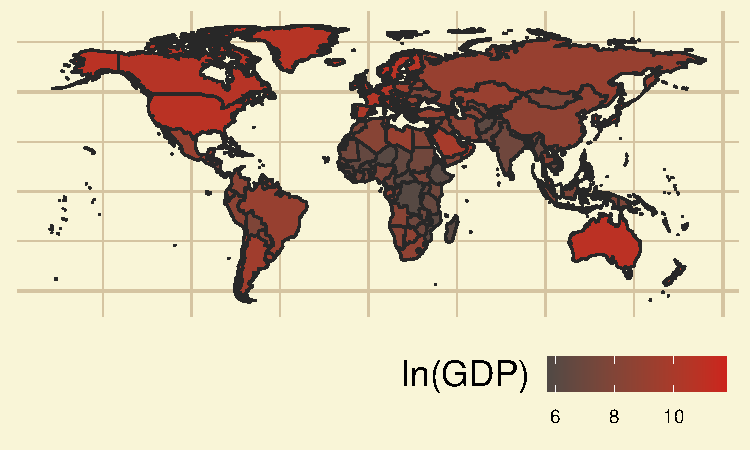
\includegraphics{main_files/figure-pdf/unnamed-chunk-3-1.pdf} \hfill{}

\end{figure}

\begin{figure}

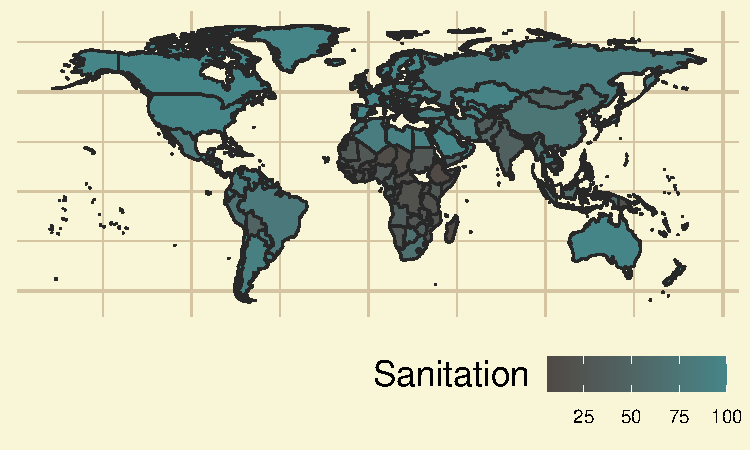
\includegraphics{main_files/figure-pdf/unnamed-chunk-4-1.pdf} \hfill{}

\end{figure}

\[
~
\]

\begin{figure}

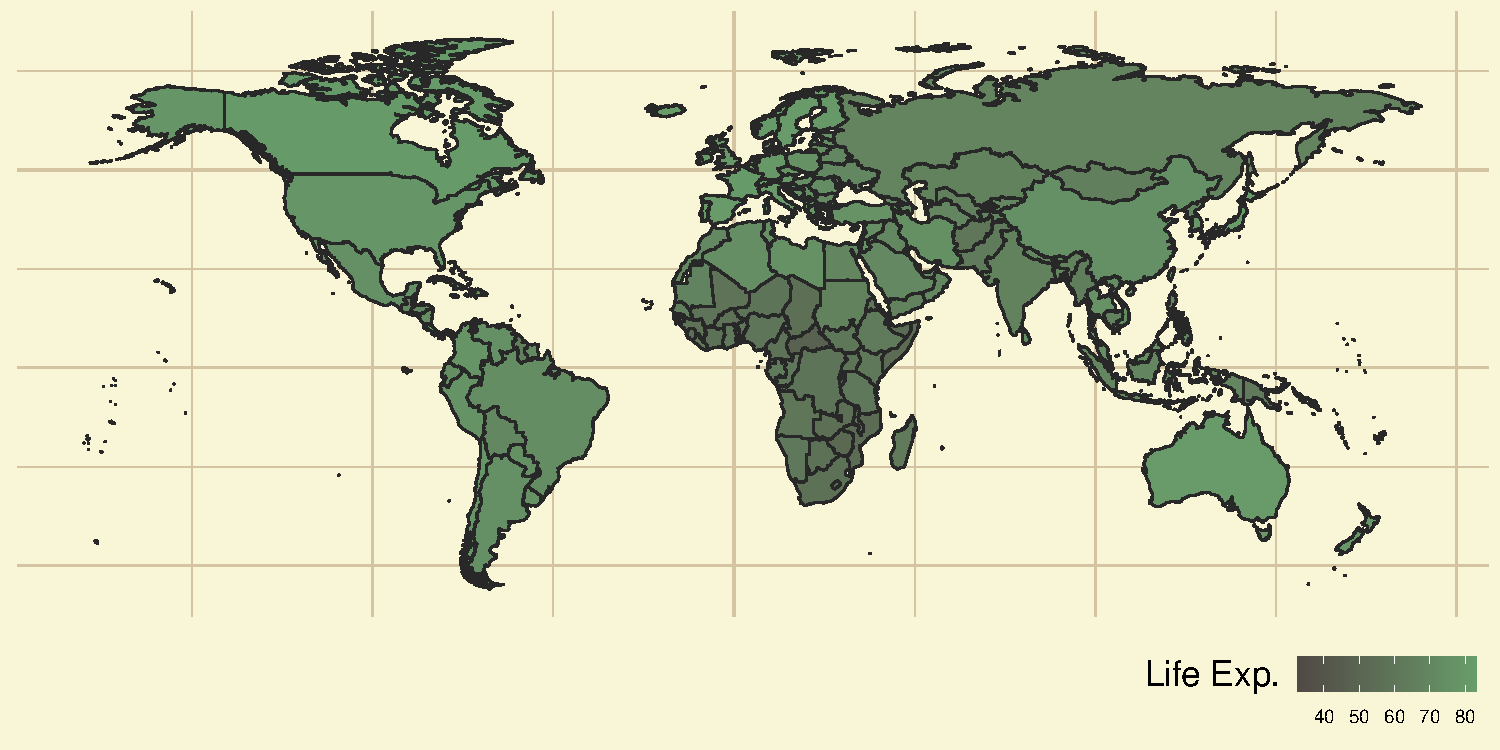
\includegraphics{main_files/figure-pdf/unnamed-chunk-5-1.pdf} \hfill{}

\end{figure}

\hypertarget{variables}: Percentage of people using at least
  basic Sanitation facilities, not shared with other households.
  {[}\emph{snt}{]}

  Sanitation of oneself is one of the basic tasks of a human being. We
  know poor sanitation is linked to transmission of diarrheal diseases
  such as cholera and dysentery, as well as typhoid, intestinal worm
  infections and polio which directly affect the health of an
  individual.
\item
  \textbf{Life Expectancy}: The average number of years a newly born
  child would live, provided current mortality patterns hold.
  {[}\emph{lfx}{]}

  Life expectancy is calculated based on the assumption that probability
  of death at a certain age stays constant in future. Hence we Life
  Expectation as a measurable proxy for Health.
\end{itemize}

\hypertarget{data}{%
\subsection{Data}\label{data}}

\begin{Shaded}
\begin{Highlighting}[]
\NormalTok{script.dir }\OtherTok{\textless{}{-}} \FunctionTok{getSrcDirectory}\NormalTok{(}\ControlFlowTok{function}\NormalTok{(x) \{x\})}
\FunctionTok{setwd}\NormalTok{(script.dir)}

\NormalTok{numerise }\OtherTok{=} \ControlFlowTok{function}\NormalTok{(x)\{}
\NormalTok{  x[}\FunctionTok{grepl}\NormalTok{(}\StringTok{"k$"}\NormalTok{, x)] }\OtherTok{\textless{}{-}} \FunctionTok{as.numeric}\NormalTok{(}\FunctionTok{sub}\NormalTok{(}\StringTok{"k$"}\NormalTok{, }\StringTok{""}\NormalTok{, x[}\FunctionTok{grepl}\NormalTok{(}\StringTok{"k$"}\NormalTok{, x)]))}\SpecialCharTok{*}\DecValTok{10}\SpecialCharTok{\^{}}\DecValTok{3}
\NormalTok{  x }\OtherTok{\textless{}{-}} \FunctionTok{as.numeric}\NormalTok{(x)}
  \FunctionTok{return}\NormalTok{(x)}
\NormalTok{\}}

\NormalTok{d1\_raw }\OtherTok{=} \FunctionTok{read.csv}\NormalTok{(}\FunctionTok{file.path}\NormalTok{(}\StringTok{"."}\NormalTok{,}\StringTok{"Data"}\NormalTok{,}\StringTok{"gdp.csv"}\NormalTok{), }\AttributeTok{fileEncoding =} \StringTok{\textquotesingle{}UTF{-}8{-}BOM\textquotesingle{}}\NormalTok{)}
\NormalTok{d2\_raw }\OtherTok{=} \FunctionTok{read.csv}\NormalTok{(}\FunctionTok{file.path}\NormalTok{(}\StringTok{"."}\NormalTok{,}\StringTok{"Data"}\NormalTok{,}\StringTok{"sanitation.csv"}\NormalTok{), }\AttributeTok{fileEncoding =} \StringTok{\textquotesingle{}UTF{-}8{-}BOM\textquotesingle{}}\NormalTok{)}
\NormalTok{d3\_raw }\OtherTok{=} \FunctionTok{read.csv}\NormalTok{(}\FunctionTok{file.path}\NormalTok{(}\StringTok{"."}\NormalTok{,}\StringTok{"Data"}\NormalTok{,}\StringTok{"life\_expectancy.csv"}\NormalTok{), }\AttributeTok{fileEncoding =} \StringTok{\textquotesingle{}UTF{-}8{-}BOM\textquotesingle{}}\NormalTok{)}

\NormalTok{yearname }\OtherTok{=} \StringTok{"X2010"}

\NormalTok{d1 }\OtherTok{=}\NormalTok{ d1\_raw[}\SpecialCharTok{!}\FunctionTok{is.na}\NormalTok{(}\FunctionTok{numerise}\NormalTok{(d1\_raw[, yearname])),][,}\FunctionTok{c}\NormalTok{(}\StringTok{"country"}\NormalTok{, yearname)]}
\FunctionTok{colnames}\NormalTok{(d1)[}\DecValTok{2}\NormalTok{] }\OtherTok{=} \StringTok{"lngdp"}
\NormalTok{d2 }\OtherTok{=}\NormalTok{ d2\_raw[}\SpecialCharTok{!}\FunctionTok{is.na}\NormalTok{(}\FunctionTok{numerise}\NormalTok{(d2\_raw[, yearname])),][,}\FunctionTok{c}\NormalTok{(}\StringTok{"country"}\NormalTok{, yearname)]}
\FunctionTok{colnames}\NormalTok{(d2)[}\DecValTok{2}\NormalTok{] }\OtherTok{=} \StringTok{"snt"}
\NormalTok{d3 }\OtherTok{=}\NormalTok{ d3\_raw[}\SpecialCharTok{!}\FunctionTok{is.na}\NormalTok{(}\FunctionTok{numerise}\NormalTok{(d3\_raw[, yearname])),][,}\FunctionTok{c}\NormalTok{(}\StringTok{"country"}\NormalTok{, yearname)]}
\FunctionTok{colnames}\NormalTok{(d3)[}\DecValTok{2}\NormalTok{] }\OtherTok{=} \StringTok{"lfx"}

\NormalTok{dtemp }\OtherTok{=} \FunctionTok{merge}\NormalTok{(}\AttributeTok{x =}\NormalTok{ d1, }\AttributeTok{y =}\NormalTok{ d2, }\AttributeTok{by =} \StringTok{"country"}\NormalTok{)}
\NormalTok{d }\OtherTok{=} \FunctionTok{merge}\NormalTok{(}\AttributeTok{x =}\NormalTok{ dtemp, }\AttributeTok{y =}\NormalTok{ d3, }\AttributeTok{by =} \StringTok{"country"}\NormalTok{)}

\NormalTok{d}\SpecialCharTok{$}\NormalTok{lngdp }\OtherTok{=} \FunctionTok{log}\NormalTok{(}\FunctionTok{numerise}\NormalTok{(d}\SpecialCharTok{$}\NormalTok{lngdp))}

\FunctionTok{write.csv}\NormalTok{(d, }\StringTok{"./Data/assembled.csv"}\NormalTok{)}

\FunctionTok{kable}\NormalTok{(}\FunctionTok{head}\NormalTok{(d, 6L))}
\end{Highlighting}
\end{Shaded}

\begin{longtable}[]{@{}lrrr@{}}
\toprule()
country & lngdp & snt & lfx \\
\midrule()
\endhead
Afghanistan & 6.265301 & 34.9 & 60.5 \\
Albania & 8.183118 & 95.2 & 78.1 \\
Algeria & 8.273847 & 87.0 & 74.5 \\
Andorra & 10.454495 & 100.0 & 81.8 \\
Angola & 8.291547 & 41.1 & 60.2 \\
Antigua and Barbuda & 9.546813 & 86.3 & 75.9 \\
\bottomrule()
\end{longtable}

\marginnote{\begin{footnotesize}

FREE DATA FROM \href{un.org}{UN}, \href{https://worldbank.org}{WORLD
BANK}, \href{https://who.org}{WHO},
\href{http://www.healthdata.org/}{IMHE} VIA
\href{https://gapminder.org}{GAPMINDER.ORG},
\href{https://creativecommons.org/licenses/by/2.0/}{CC-BY LICENSE}.

\end{footnotesize}}

\hypertarget{elementary-univariate-analysis}{%
\section{Elementary Univariate
Analysis}\label{elementary-univariate-analysis}}

\hypertarget{measures-of-central-tendency}{%
\subsection{Measures of Central
Tendency}\label{measures-of-central-tendency}}

\emph{Mean or Arithmetic Mean} \(\bar{x}\), \emph{Median}
\(\operatorname{median}(x)\) and \emph{Mode} \(\operatorname{mode}(x)\)
are some measures of \emph{central tendency} in the sample.

Formulae

\[
\begin{aligned}
x = \{x_1, x_2, \ldots,x_{n-1}, x_n\} &&
\operatorname{mean}(x)=\bar{x} = \frac{1}{n} \sum _{i=1}^{n}(x_{i})
\end{aligned}
\]\[
\begin{aligned}
\operatorname{median}(x)= \frac{x_{\lfloor\frac{n+1}{2}\rfloor}+x_{\lfloor\frac{n+2}{2}\rfloor}}{2} &&
\operatorname{mode}(x) = x_i \text{ s.t. } \operatorname{Pr}(x_i) = \operatorname{sup}(\operatorname{Pr}(x))  
\end{aligned}
\]

Note: \(f_i\) is the frequency of the ith observation. \(x_{(i)}\) is
the ith largest observation.

\begin{Shaded}
\begin{Highlighting}[]
\NormalTok{getmode }\OtherTok{\textless{}{-}} \ControlFlowTok{function}\NormalTok{(v) \{}
\NormalTok{ uniqv }\OtherTok{\textless{}{-}} \FunctionTok{unique}\NormalTok{(v)}
\NormalTok{ freq }\OtherTok{=} \FunctionTok{max}\NormalTok{(}\FunctionTok{tabulate}\NormalTok{(}\FunctionTok{match}\NormalTok{(v, uniqv)))}
\NormalTok{ res }\OtherTok{=}\NormalTok{ uniqv[}\FunctionTok{which.max}\NormalTok{(}\FunctionTok{tabulate}\NormalTok{(}\FunctionTok{match}\NormalTok{(v, uniqv)))]}
 \ControlFlowTok{if}\NormalTok{ (freq }\SpecialCharTok{==} \DecValTok{1}\NormalTok{) res }\OtherTok{=} \ConstantTok{NULL}
 \FunctionTok{return}\NormalTok{(res)}
\NormalTok{\}}

\NormalTok{d\_central }\OtherTok{=} \FunctionTok{data.frame}\NormalTok{(}
  \AttributeTok{row.names =} \StringTok{"Variable"}\NormalTok{,}
  \AttributeTok{Variable =} \FunctionTok{c}\NormalTok{(}
    \StringTok{"*ln(GDP)*"}\NormalTok{,}
    \StringTok{"*Sanitation*"}\NormalTok{,}
    \StringTok{"*Life Exp.*"}
\NormalTok{  ),}
  \AttributeTok{Mean =} \FunctionTok{c}\NormalTok{(}
    \FunctionTok{mean}\NormalTok{(d}\SpecialCharTok{$}\NormalTok{lngdp),}
    \FunctionTok{mean}\NormalTok{(d}\SpecialCharTok{$}\NormalTok{snt),}
    \FunctionTok{mean}\NormalTok{(d}\SpecialCharTok{$}\NormalTok{lfx)}
\NormalTok{  ),}
  \AttributeTok{Median =} \FunctionTok{c}\NormalTok{(}
    \FunctionTok{median}\NormalTok{(d}\SpecialCharTok{$}\NormalTok{lngdp),}
    \FunctionTok{median}\NormalTok{(d}\SpecialCharTok{$}\NormalTok{snt),}
    \FunctionTok{median}\NormalTok{(d}\SpecialCharTok{$}\NormalTok{lfx)}
\NormalTok{  ),}
  \AttributeTok{Mode =} \FunctionTok{c}\NormalTok{(}
    \FunctionTok{getmode}\NormalTok{(d}\SpecialCharTok{$}\NormalTok{lngdp),}
    \FunctionTok{getmode}\NormalTok{(d}\SpecialCharTok{$}\NormalTok{snt),}
    \FunctionTok{getmode}\NormalTok{(d}\SpecialCharTok{$}\NormalTok{lfx)}
\NormalTok{  )}
\NormalTok{)}

\FunctionTok{kable}\NormalTok{(}
\NormalTok{  d\_central,}
  \AttributeTok{col.names =} \FunctionTok{c}\NormalTok{(}
    \StringTok{"$}\SpecialCharTok{\textbackslash{}\textbackslash{}}\StringTok{quad }\SpecialCharTok{\textbackslash{}\textbackslash{}}\StringTok{quad }\SpecialCharTok{\textbackslash{}\textbackslash{}}\StringTok{bar\{x\}$"}\NormalTok{,}
    \StringTok{"$}\SpecialCharTok{\textbackslash{}\textbackslash{}}\StringTok{operatorname\{median\}(x)$"}\NormalTok{,}
    \StringTok{"$}\SpecialCharTok{\textbackslash{}\textbackslash{}}\StringTok{operatorname\{mode\}(x)$"}
\NormalTok{  ),}
  \AttributeTok{digits=}\DecValTok{5}
\NormalTok{)}
\end{Highlighting}
\end{Shaded}

\begin{longtable}[]{@{}
  >{\raggedright\arraybackslash}p{(\columnwidth - 6\tabcolsep) * \real{0.1494}}
  >{\raggedleft\arraybackslash}p{(\columnwidth - 6\tabcolsep) * \real{0.2529}}
  >{\raggedleft\arraybackslash}p{(\columnwidth - 6\tabcolsep) * \real{0.3103}}
  >{\raggedleft\arraybackslash}p{(\columnwidth - 6\tabcolsep) * \real{0.2874}}@{}}
\toprule()
\begin{minipage}[b]{\linewidth}\raggedright
\end{minipage} & \begin{minipage}[b]{\linewidth}\raggedleft
\(\quad \quad \bar{x}\)
\end{minipage} & \begin{minipage}[b]{\linewidth}\raggedleft
\(\operatorname{median}(x)\)
\end{minipage} & \begin{minipage}[b]{\linewidth}\raggedleft
\(\operatorname{mode}(x)\)
\end{minipage} \\
\midrule()
\endhead
\emph{ln(GDP)} & 8.54124 & 8.48673 & 9.23014 \\
\emph{Sanitation} & 72.43857 & 85.60000 & 100.00000 \\
\emph{Life Exp.} & 70.54603 & 72.40000 & 73.20000 \\
\bottomrule()
\end{longtable}

\(~\)

\begin{itemize}
\tightlist
\item
  Notice that mode of Sanitation is 100. Thus a large number of
  countries have universal access to basic sanitation infrastructure.
\end{itemize}

\hypertarget{measures-of-dispersion}{%
\subsection{Measures of Dispersion}\label{measures-of-dispersion}}

\emph{Range} \(\operatorname{range}(x)\), \emph{Semi-Interquartile
Range} \(\operatorname{SIR}(x)\), \emph{Mean Deviation about x'}
\(\operatorname{MD}_{(x')}(x)\), \emph{Variance} \(s_x^2\),
\emph{Standard Deviation} \(s_x\) are some measures of \emph{dispersion}
in the sample.

Formulae

\[
\begin{aligned}
\operatorname{range}(x)=|x_{(n)} - x_{(1)}| &&
\ Q_1 = \operatorname{median}(x_{(1)}, \ldots ,x_{(\lfloor \frac{n+1}{2} \rfloor)}) &&
\end{aligned}
\] \[
\begin{aligned}
\ Q_3 = \operatorname{median}(x_{(\lfloor \frac{n+2}{2} \rfloor)}, \ldots , x_{(n)}) &&
\operatorname{MD}_{(x')}(x) = \operatorname{mean}(|x_i-x'|)
\end{aligned}
\] \[
\begin{aligned}
\operatorname{SIR}(x)=\frac{|Q_1-Q_3|}{2} &&
s_x = \sqrt{\operatorname{mean}([x_i - \bar{x}]^2)} &&
s^2_x= (s_x)^2
\end{aligned}
\]

\begin{Shaded}
\begin{Highlighting}[]
\NormalTok{getmd }\OtherTok{=} \ControlFlowTok{function}\NormalTok{(x, }\AttributeTok{center =} \FunctionTok{mean}\NormalTok{(x))\{}
\NormalTok{  md }\OtherTok{=} \FunctionTok{mean}\NormalTok{(}
    \FunctionTok{abs}\NormalTok{(}
\NormalTok{      x }\SpecialCharTok{{-}} \FunctionTok{rep}\NormalTok{(center, }\FunctionTok{length}\NormalTok{(x))}
\NormalTok{      )}
\NormalTok{    )}
  \FunctionTok{return}\NormalTok{(md)}
\NormalTok{\}}
\NormalTok{d\_disp }\OtherTok{=} \FunctionTok{data.frame}\NormalTok{(}
  \AttributeTok{row.names =} \StringTok{"Variable"}\NormalTok{,}
  \AttributeTok{Variable =} \FunctionTok{c}\NormalTok{(}
    \StringTok{"*ln(GDP)*"}\NormalTok{,}
    \StringTok{"*Sanitation*"}\NormalTok{,}
    \StringTok{"*Life Exp.*"}
\NormalTok{  ),}
  \AttributeTok{Range =} \FunctionTok{c}\NormalTok{(}
    \FunctionTok{max}\NormalTok{(d}\SpecialCharTok{$}\NormalTok{lngdp) }\SpecialCharTok{{-}} \FunctionTok{min}\NormalTok{(d}\SpecialCharTok{$}\NormalTok{lngdp),}
    \FunctionTok{max}\NormalTok{(d}\SpecialCharTok{$}\NormalTok{snt) }\SpecialCharTok{{-}} \FunctionTok{min}\NormalTok{(d}\SpecialCharTok{$}\NormalTok{snt),}
    \FunctionTok{max}\NormalTok{(d}\SpecialCharTok{$}\NormalTok{lfx) }\SpecialCharTok{{-}} \FunctionTok{min}\NormalTok{(d}\SpecialCharTok{$}\NormalTok{lfx)}
\NormalTok{  ),}
  \AttributeTok{SIR =} \FunctionTok{c}\NormalTok{(}
    \FunctionTok{IQR}\NormalTok{(d}\SpecialCharTok{$}\NormalTok{lngdp)}\SpecialCharTok{/}\DecValTok{2}\NormalTok{,}
    \FunctionTok{IQR}\NormalTok{(d}\SpecialCharTok{$}\NormalTok{snt)}\SpecialCharTok{/}\DecValTok{2}\NormalTok{,}
    \FunctionTok{IQR}\NormalTok{(d}\SpecialCharTok{$}\NormalTok{lfx)}\SpecialCharTok{/}\DecValTok{2}
\NormalTok{  ),}
  \AttributeTok{MD =} \FunctionTok{c}\NormalTok{(}
    \FunctionTok{getmd}\NormalTok{(d}\SpecialCharTok{$}\NormalTok{lngdp),}
    \FunctionTok{getmd}\NormalTok{(d}\SpecialCharTok{$}\NormalTok{snt),}
    \FunctionTok{getmd}\NormalTok{(d}\SpecialCharTok{$}\NormalTok{lfx)}
\NormalTok{  ),}
  \AttributeTok{variance =} \FunctionTok{c}\NormalTok{(}
\NormalTok{    (}\FunctionTok{sd}\NormalTok{(d}\SpecialCharTok{$}\NormalTok{lngdp))}\SpecialCharTok{\^{}}\DecValTok{2}\NormalTok{,}
\NormalTok{    (}\FunctionTok{sd}\NormalTok{(d}\SpecialCharTok{$}\NormalTok{snt))}\SpecialCharTok{\^{}}\DecValTok{2}\NormalTok{,}
\NormalTok{    (}\FunctionTok{sd}\NormalTok{(d}\SpecialCharTok{$}\NormalTok{lfx))}\SpecialCharTok{\^{}}\DecValTok{2}
\NormalTok{  ),}
  \AttributeTok{SD =} \FunctionTok{c}\NormalTok{(}
    \FunctionTok{sd}\NormalTok{(d}\SpecialCharTok{$}\NormalTok{lngdp),}
    \FunctionTok{sd}\NormalTok{(d}\SpecialCharTok{$}\NormalTok{snt),}
    \FunctionTok{sd}\NormalTok{(d}\SpecialCharTok{$}\NormalTok{lfx)}
\NormalTok{  )}
\NormalTok{)}

\FunctionTok{kable}\NormalTok{(}
\NormalTok{  d\_disp,}
  \AttributeTok{col.names =} \FunctionTok{c}\NormalTok{(}
    \StringTok{"$}\SpecialCharTok{\textbackslash{}\textbackslash{}}\StringTok{operatorname\{range\}(x)$"}\NormalTok{,}
    \StringTok{"$}\SpecialCharTok{\textbackslash{}\textbackslash{}}\StringTok{operatorname\{SIR\}(x)$"}\NormalTok{,}
    \StringTok{"$}\SpecialCharTok{\textbackslash{}\textbackslash{}}\StringTok{operatorname\{MD\}\_\{(}\SpecialCharTok{\textbackslash{}\textbackslash{}}\StringTok{bar\{x\})\}(x)$"}\NormalTok{,}
    \StringTok{"$}\SpecialCharTok{\textbackslash{}\textbackslash{}}\StringTok{quad }\SpecialCharTok{\textbackslash{}\textbackslash{}}\StringTok{quad }\SpecialCharTok{\textbackslash{}\textbackslash{}}\StringTok{quad }\SpecialCharTok{\textbackslash{}\textbackslash{}}\StringTok{quad s\_x\^{}2$"}\NormalTok{,}
    \StringTok{"$}\SpecialCharTok{\textbackslash{}\textbackslash{}}\StringTok{quad }\SpecialCharTok{\textbackslash{}\textbackslash{}}\StringTok{quad }\SpecialCharTok{\textbackslash{}\textbackslash{}}\StringTok{quad }\SpecialCharTok{\textbackslash{}\textbackslash{}}\StringTok{quad s\_x$"}
\NormalTok{  ),}
  \AttributeTok{digits=}\DecValTok{5}
\NormalTok{)}
\end{Highlighting}
\end{Shaded}

\begin{longtable}[]{@{}
  >{\raggedright\arraybackslash}p{(\columnwidth - 10\tabcolsep) * \real{0.0812}}
  >{\raggedleft\arraybackslash}p{(\columnwidth - 10\tabcolsep) * \real{0.1625}}
  >{\raggedleft\arraybackslash}p{(\columnwidth - 10\tabcolsep) * \real{0.1500}}
  >{\raggedleft\arraybackslash}p{(\columnwidth - 10\tabcolsep) * \real{0.2188}}
  >{\raggedleft\arraybackslash}p{(\columnwidth - 10\tabcolsep) * \real{0.2000}}
  >{\raggedleft\arraybackslash}p{(\columnwidth - 10\tabcolsep) * \real{0.1875}}@{}}
\toprule()
\begin{minipage}[b]{\linewidth}\raggedright
\end{minipage} & \begin{minipage}[b]{\linewidth}\raggedleft
\(\operatorname{range}(x)\)
\end{minipage} & \begin{minipage}[b]{\linewidth}\raggedleft
\(\operatorname{SIR}(x)\)
\end{minipage} & \begin{minipage}[b]{\linewidth}\raggedleft
\(\operatorname{MD}_{(\bar{x})}(x)\)
\end{minipage} & \begin{minipage}[b]{\linewidth}\raggedleft
\(\quad \quad \quad \quad s_x^2\)
\end{minipage} & \begin{minipage}[b]{\linewidth}\raggedleft
\(\quad \quad \quad \quad s_x\)
\end{minipage} \\
\midrule()
\endhead
\emph{ln(GDP)} & 6.04435 & 1.06914 & 1.17229 & 2.01791 & 1.42053 \\
\emph{Sanitation} & 94.03000 & 24.65000 & 25.50487 & 872.29346 &
29.53461 \\
\emph{Life Exp.} & 50.80000 & 6.00000 & 6.98712 & 75.33494 & 8.67957 \\
\bottomrule()
\end{longtable}

\(~\)

\begin{itemize}
\tightlist
\item
  We can compare \(s_x\) to \(\bar{x}\) and observe that there is a high
  variation in Sanitation amongst countries.
\item
  GDP per capita varies drastically across the \(e\)6.044354 range.
\end{itemize}

\hypertarget{measures-of-shape}{%
\subsection{Measures of Shape}\label{measures-of-shape}}

Coefficients of \emph{Skewness} \(g_1\) and \emph{Kurtosis} \(g_2\)
describe the symmetry and extremity of tails of the sample distribution.

Formulae

\[
\begin{aligned}
m_k = \operatorname{mean}([x-\bar{x}]^k) &&
g_1 = \frac{m_3}{{m_2}^{\frac{3}{2}}} &&
g_2 = \frac{m_4}{{m_2}^2}
\end{aligned}
\]

\begin{Shaded}
\begin{Highlighting}[]
\NormalTok{d\_shape }\OtherTok{=} \FunctionTok{data.frame}\NormalTok{(}
  \AttributeTok{row.names =} \StringTok{"Variable"}\NormalTok{,}
  \AttributeTok{Variable =} \FunctionTok{c}\NormalTok{(}
    \StringTok{"*ln(GDP)*"}\NormalTok{,}
    \StringTok{"*Sanitation*"}\NormalTok{,}
    \StringTok{"*Life Exp.*"}
\NormalTok{  ),}
  \AttributeTok{Skewness =} \FunctionTok{c}\NormalTok{(}
    \FunctionTok{skewness}\NormalTok{(d}\SpecialCharTok{$}\NormalTok{lngdp),}
    \FunctionTok{skewness}\NormalTok{(d}\SpecialCharTok{$}\NormalTok{snt),}
    \FunctionTok{skewness}\NormalTok{(d}\SpecialCharTok{$}\NormalTok{lfx)}
\NormalTok{  ),}
  \AttributeTok{Kurtosis =} \FunctionTok{c}\NormalTok{(}
    \FunctionTok{kurtosis}\NormalTok{(d}\SpecialCharTok{$}\NormalTok{lngdp),}
    \FunctionTok{kurtosis}\NormalTok{(d}\SpecialCharTok{$}\NormalTok{snt),}
    \FunctionTok{kurtosis}\NormalTok{(d}\SpecialCharTok{$}\NormalTok{lfx)}
\NormalTok{  )}
\NormalTok{)}

\FunctionTok{kable}\NormalTok{(}
\NormalTok{  d\_shape,}
  \AttributeTok{col.names =} \FunctionTok{c}\NormalTok{(}
    \StringTok{"Skewness $g\_1$"}\NormalTok{,}
    \StringTok{"Kurtosis $g\_2$"}
\NormalTok{  ),}
  \AttributeTok{digits=}\DecValTok{5}
\NormalTok{)}
\end{Highlighting}
\end{Shaded}

\begin{longtable}[]{@{}lrr@{}}
\toprule()
& Skewness \(g_1\) & Kurtosis \(g_2\) \\
\midrule()
\endhead
\emph{ln(GDP)} & 0.09619 & 2.14435 \\
\emph{Sanitation} & -0.85989 & 2.27111 \\
\emph{Life Exp.} & -0.87903 & 4.02465 \\
\bottomrule()
\end{longtable}

\[
~
\]

\begin{itemize}
\item
  ln(GDP) is nearly symmetrical, while Sanitation and Life Exp. are
  highly left-skewed.

  This indicates majority of countries have good sanitation system and
  citizen health.
\item
  ln(GDP) and Sanitation are platykurtic, while Life Exp. is
  leptokurtic.
\end{itemize}

\hypertarget{density-plot}{%
\subsection{Density Plot}\label{density-plot}}

\begin{Shaded}
\begin{Highlighting}[]
\NormalTok{labelfunction }\OtherTok{=} \FunctionTok{as\_labeller}\NormalTok{(}\FunctionTok{c}\NormalTok{(}
    \StringTok{\textasciigrave{}}\AttributeTok{lngdp}\StringTok{\textasciigrave{}} \OtherTok{=} \StringTok{"log of GDP per capita"}\NormalTok{,}
    \StringTok{\textasciigrave{}}\AttributeTok{snt}\StringTok{\textasciigrave{}} \OtherTok{=} \StringTok{"Sanitation Access \%"}\NormalTok{,}
    \StringTok{\textasciigrave{}}\AttributeTok{lfx}\StringTok{\textasciigrave{}} \OtherTok{=} \StringTok{"Life Expectancy"}
\NormalTok{    )}
\NormalTok{)}

\FunctionTok{ggplot}\NormalTok{(}\FunctionTok{stack}\NormalTok{(d[}\DecValTok{2}\SpecialCharTok{:}\DecValTok{4}\NormalTok{]), }\AttributeTok{mapping =} \FunctionTok{aes}\NormalTok{(}\AttributeTok{x =}\NormalTok{ values))}\SpecialCharTok{+}
\FunctionTok{geom\_density}\NormalTok{(}\FunctionTok{aes}\NormalTok{(}\AttributeTok{color=}\NormalTok{ind), }\AttributeTok{linewidth=}\FunctionTok{rel}\NormalTok{(}\FloatTok{1.5}\NormalTok{))}\SpecialCharTok{+}
\FunctionTok{labs}\NormalTok{(}
  \AttributeTok{x=}\ConstantTok{NULL}\NormalTok{,}
  \AttributeTok{y=}\ConstantTok{NULL}
\NormalTok{  )}\SpecialCharTok{+}
\NormalTok{mytheme}\SpecialCharTok{+}
\NormalTok{mycolor}\SpecialCharTok{+}
\FunctionTok{facet\_wrap}\NormalTok{(}\SpecialCharTok{\textasciitilde{}}\NormalTok{ind, }\AttributeTok{scales=}\StringTok{"free"}\NormalTok{, }\AttributeTok{labeller =}\NormalTok{ labelfunction, }\AttributeTok{ncol=}\DecValTok{1}\NormalTok{)}\SpecialCharTok{+}
  \FunctionTok{theme}\NormalTok{(}\AttributeTok{legend.position=}\StringTok{"none"}\NormalTok{,}
        \AttributeTok{strip.text.x =} \FunctionTok{element\_text}\NormalTok{(}\AttributeTok{size =} \FunctionTok{rel}\NormalTok{(}\FloatTok{1.5}\NormalTok{))}
\NormalTok{  )}
\end{Highlighting}
\end{Shaded}

\begin{figure}[H]

{\centering 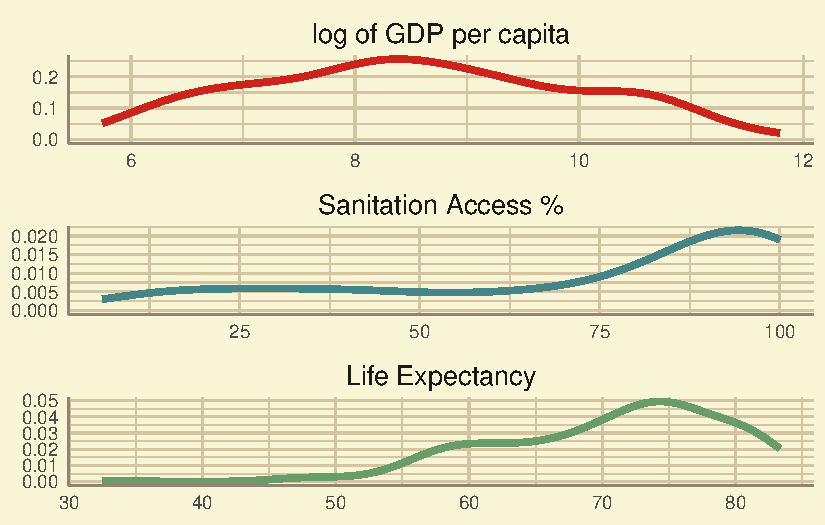
\includegraphics{main_files/figure-pdf/unnamed-chunk-10-1.pdf}

}

\end{figure}

\begin{itemize}
\tightlist
\item
  The density of the log of GDP per capita is symmetric as inferred
  previously. The other two density plots appear left skewed as
  supported by the negative skewness.
\end{itemize}

\hypertarget{box-plot}{%
\subsection{Box Plot}\label{box-plot}}

\emph{Box plots} help us detect potential outliers. They also help us in
estimating location and skewness of the distribution.

\begin{Shaded}
\begin{Highlighting}[]
\NormalTok{plot1 }\OtherTok{=} \FunctionTok{ggplot}\NormalTok{(}\FunctionTok{stack}\NormalTok{(d[}\DecValTok{2}\SpecialCharTok{:}\DecValTok{4}\NormalTok{]), }\AttributeTok{mapping =} \FunctionTok{aes}\NormalTok{(}\AttributeTok{y =}\NormalTok{ values, }\AttributeTok{x =}\NormalTok{ ind))}\SpecialCharTok{+}
\FunctionTok{geom\_boxplot}\NormalTok{(}\FunctionTok{aes}\NormalTok{(}\AttributeTok{fill=}\NormalTok{ind), }\AttributeTok{alpha=}\FloatTok{0.6}\NormalTok{)}\SpecialCharTok{+}
\FunctionTok{labs}\NormalTok{(}
  \AttributeTok{x=}\ConstantTok{NULL}\NormalTok{,}
  \AttributeTok{y=}\ConstantTok{NULL}
\NormalTok{  )}\SpecialCharTok{+}
\NormalTok{mytheme}\SpecialCharTok{+}
\FunctionTok{facet\_wrap}\NormalTok{(}\FunctionTok{vars}\NormalTok{(ind), }\AttributeTok{scales=}\StringTok{"free"}\NormalTok{, }\AttributeTok{labeller =}\NormalTok{ labelfunction)}\SpecialCharTok{+}
  \FunctionTok{theme}\NormalTok{(}\AttributeTok{axis.text.x=}\FunctionTok{element\_blank}\NormalTok{(),}
        \AttributeTok{legend.position=}\StringTok{"none"}\NormalTok{,}
        \AttributeTok{strip.text.x =} \FunctionTok{element\_text}\NormalTok{(}\AttributeTok{size =} \FunctionTok{rel}\NormalTok{(}\FloatTok{1.5}\NormalTok{)),}
        \AttributeTok{panel.grid.minor.x =} \FunctionTok{element\_blank}\NormalTok{(),}
        \AttributeTok{panel.grid.major.x =} \FunctionTok{element\_blank}\NormalTok{()}
\NormalTok{  )}\SpecialCharTok{+}
  \FunctionTok{scale\_color\_manual}\NormalTok{(}
      \AttributeTok{values=}\FunctionTok{c}\NormalTok{(}
        \StringTok{"\#cc241d"}\NormalTok{,}
        \StringTok{"\#458588"}\NormalTok{,}
        \StringTok{"\#689d6a"}\NormalTok{,}
        \StringTok{"\#d65d0e"}
\NormalTok{        ),}
      \AttributeTok{aesthetics=}\StringTok{"fill"}
\NormalTok{      )}


\FunctionTok{ggplotly}\NormalTok{(plot1)}
\end{Highlighting}
\end{Shaded}

\begin{itemize}
\tightlist
\item
  We observe one potential outlier in the Life Expectancy dataset. It is
  Haiti at 32.5 years. It is due to a cholera outbreak and an earthquake
  increasing the mortality rate in the nation in 2010.
\end{itemize}

\hypertarget{scatter-plot}{%
\section{Scatter Plot}\label{scatter-plot}}

A \emph{Scatter plot} helps us estimate the type of relationship between
variables.

\begin{Shaded}
\begin{Highlighting}[]
\NormalTok{sctrplot }\OtherTok{=} \ControlFlowTok{function}\NormalTok{(}
\NormalTok{    d, x\_map, y\_map,}
    \AttributeTok{x\_lab=}\FunctionTok{waiver}\NormalTok{(), }\AttributeTok{y\_lab=}\FunctionTok{waiver}\NormalTok{(),}
    \AttributeTok{title=}\FunctionTok{waiver}\NormalTok{()}
\NormalTok{)\{}
\NormalTok{  plot1 }\OtherTok{=} \FunctionTok{ggplot}\NormalTok{(d, }\AttributeTok{mapping =} \FunctionTok{aes}\NormalTok{(}\AttributeTok{x =}\NormalTok{ x\_map, }\AttributeTok{y =}\NormalTok{ y\_map, }\AttributeTok{text =}\NormalTok{ country))}\SpecialCharTok{+}
    \FunctionTok{geom\_point}\NormalTok{(}
      \AttributeTok{alpha=}\FloatTok{0.6}
\NormalTok{    )}\SpecialCharTok{+}
\NormalTok{    mytheme}\SpecialCharTok{+}
    \FunctionTok{labs}\NormalTok{(}
      \AttributeTok{x=}\NormalTok{x\_lab,}
      \AttributeTok{y=}\NormalTok{y\_lab,}
      \AttributeTok{title=}\NormalTok{title}
\NormalTok{    )}
  
\NormalTok{  plot2 }\OtherTok{=} \FunctionTok{ggplotly}\NormalTok{(plot1,}
                   \AttributeTok{tooltip =} \StringTok{"text"}\NormalTok{)}
  \FunctionTok{return}\NormalTok{(plot2)}
\NormalTok{\}}
\end{Highlighting}
\end{Shaded}

\hypertarget{sanitation-vs.-log-of-gdp}{%
\subsection{Sanitation vs.~log of GDP}\label{sanitation-vs.-log-of-gdp}}

\begin{itemize}
\tightlist
\item
  We observe from the scatter plot that the correlation between ln(GDP)
  and sanitation access appears to be mostly Linear for countries with
  low ln(GDP).
\item
  Also, the sanitation access is very close to 100\% for countries with
  high ln(GDP).
\end{itemize}

\hypertarget{life-expectancy-vs.-log-of-gdp}{%
\subsection{Life Expectancy vs.~log of
GDP}\label{life-expectancy-vs.-log-of-gdp}}

\begin{itemize}
\tightlist
\item
  We can see that except for some countries with very low life
  expectancies, the correlation between the variables is appearing to be
  linear.
\end{itemize}

\hypertarget{life-expectation-vs.-sanitation}{%
\subsection{Life Expectation
vs.~Sanitation}\label{life-expectation-vs.-sanitation}}

\begin{itemize}
\tightlist
\item
  We can see that the correlation appears to be linear between life
  expectation and sanitation. We also observe that there is clustering
  around the top right side of the plot, which is supported by the box
  plots of both the distributions.
\end{itemize}

\begin{center}\rule{0.5\linewidth}{0.5pt}\end{center}

\hypertarget{inferences}{%
\subsubsection{Inferences}\label{inferences}}

We observe a fairly strong positive Linear Correlation between the three
features in the Scatter Plot.

We subsequently compute the Correlation Coefficients to quantify the
Linear Correlation.

\hypertarget{bivariate-statistics}{%
\section{Bivariate Statistics}\label{bivariate-statistics}}

\hypertarget{correlation-coefficients}{%
\subsection{Correlation Coefficients}\label{correlation-coefficients}}

\emph{Correlation} is any relationship, causal or spurious, between two
random variables \(x\), \(y\).

\emph{Pearson's} \(r\), \emph{Spearman's} \(r_s\), and \emph{Kendall's}
\(\tau\) are some correlation coefficients. These estimate the linear
correlation between two variables.

\begin{Shaded}
\begin{Highlighting}[]
\NormalTok{d\_cor }\OtherTok{=} \FunctionTok{data.frame}\NormalTok{(}
  \AttributeTok{row.names =} \StringTok{"Variable"}\NormalTok{,}
  \AttributeTok{Variable =} \FunctionTok{c}\NormalTok{(}
    \StringTok{"*Sanitation vs. ln(GDP)*"}\NormalTok{,}
    \StringTok{"*Life Exp. vs. ln(GDP)*"}\NormalTok{,}
    \StringTok{"*Life Exp. vs. Sanitation*"}
\NormalTok{  ),}
  \AttributeTok{Pearson =} \FunctionTok{c}\NormalTok{(}
    \FunctionTok{cor}\NormalTok{(d}\SpecialCharTok{$}\NormalTok{snt, d}\SpecialCharTok{$}\NormalTok{lngdp, }\AttributeTok{method=}\StringTok{"pearson"}\NormalTok{),}
    \FunctionTok{cor}\NormalTok{(d}\SpecialCharTok{$}\NormalTok{lfx, d}\SpecialCharTok{$}\NormalTok{lngdp, }\AttributeTok{method=}\StringTok{"pearson"}\NormalTok{),}
    \FunctionTok{cor}\NormalTok{(d}\SpecialCharTok{$}\NormalTok{lfx, d}\SpecialCharTok{$}\NormalTok{snt, }\AttributeTok{method=}\StringTok{"pearson"}\NormalTok{)}
\NormalTok{  ),}
  \AttributeTok{Spearman =} \FunctionTok{c}\NormalTok{(}
    \FunctionTok{cor}\NormalTok{(d}\SpecialCharTok{$}\NormalTok{snt, d}\SpecialCharTok{$}\NormalTok{lngdp, }\AttributeTok{method=}\StringTok{"spearman"}\NormalTok{),}
    \FunctionTok{cor}\NormalTok{(d}\SpecialCharTok{$}\NormalTok{lfx, d}\SpecialCharTok{$}\NormalTok{lngdp, }\AttributeTok{method=}\StringTok{"spearman"}\NormalTok{),}
    \FunctionTok{cor}\NormalTok{(d}\SpecialCharTok{$}\NormalTok{lfx, d}\SpecialCharTok{$}\NormalTok{snt, }\AttributeTok{method=}\StringTok{"spearman"}\NormalTok{)}
\NormalTok{  ),}
  \AttributeTok{Kendall =} \FunctionTok{c}\NormalTok{(}
    \FunctionTok{cor}\NormalTok{(d}\SpecialCharTok{$}\NormalTok{snt, d}\SpecialCharTok{$}\NormalTok{lngdp, }\AttributeTok{method=}\StringTok{"kendall"}\NormalTok{),}
    \FunctionTok{cor}\NormalTok{(d}\SpecialCharTok{$}\NormalTok{lfx, d}\SpecialCharTok{$}\NormalTok{lngdp, }\AttributeTok{method=}\StringTok{"kendall"}\NormalTok{),}
    \FunctionTok{cor}\NormalTok{(d}\SpecialCharTok{$}\NormalTok{lfx, d}\SpecialCharTok{$}\NormalTok{snt, }\AttributeTok{method=}\StringTok{"kendall"}\NormalTok{)}
\NormalTok{  )}
\NormalTok{)}

\NormalTok{avg\_cor }\OtherTok{=} \FunctionTok{round}\NormalTok{(}\FunctionTok{mean}\NormalTok{(d\_cor[, }\DecValTok{1}\NormalTok{]), }\AttributeTok{digits=}\DecValTok{2}\NormalTok{)}

\FunctionTok{kable}\NormalTok{(}
\NormalTok{  d\_cor,}
  \AttributeTok{digit =} \DecValTok{5}\NormalTok{,}
  \AttributeTok{col.names =} \FunctionTok{c}\NormalTok{(}
    \StringTok{"*Pearson\textquotesingle{}s* $r$"}\NormalTok{,}
    \StringTok{"*Spearman\textquotesingle{}s* $r\_s$"}\NormalTok{,}
    \StringTok{"*Kendall\textquotesingle{}s* $}\SpecialCharTok{\textbackslash{}\textbackslash{}}\StringTok{tau$"}
\NormalTok{  )}
\NormalTok{)}
\end{Highlighting}
\end{Shaded}

\begin{longtable}[]{@{}
  >{\raggedright\arraybackslash}p{(\columnwidth - 6\tabcolsep) * \real{0.3333}}
  >{\raggedleft\arraybackslash}p{(\columnwidth - 6\tabcolsep) * \real{0.1975}}
  >{\raggedleft\arraybackslash}p{(\columnwidth - 6\tabcolsep) * \real{0.2346}}
  >{\raggedleft\arraybackslash}p{(\columnwidth - 6\tabcolsep) * \real{0.2346}}@{}}
\toprule()
\begin{minipage}[b]{\linewidth}\raggedright
\end{minipage} & \begin{minipage}[b]{\linewidth}\raggedleft
\emph{Pearson's} \(r\)
\end{minipage} & \begin{minipage}[b]{\linewidth}\raggedleft
\emph{Spearman's} \(r_s\)
\end{minipage} & \begin{minipage}[b]{\linewidth}\raggedleft
\emph{Kendall's} \(\tau\)
\end{minipage} \\
\midrule()
\endhead
\emph{Sanitation vs.~ln(GDP)} & 0.80659 & 0.85920 & 0.67458 \\
\emph{Life Exp. vs.~ln(GDP)} & 0.77229 & 0.81639 & 0.62168 \\
\emph{Life Exp. vs.~Sanitation} & 0.81351 & 0.83513 & 0.63744 \\
\bottomrule()
\end{longtable}

\[
~
\]

\begin{itemize}
\tightlist
\item
  We observe a positive correlation between all the three variables.
\item
  The correlation coefficients are close to +1, thus the correlation is
  strong.
\end{itemize}

\hypertarget{covariance-and-correlation-matrices}{%
\subsection{Covariance and Correlation
Matrices}\label{covariance-and-correlation-matrices}}

\emph{Covariance} \(\operatorname{cov}(x, y)\) is a measure of the joint
variability of two random variables \(x\), \(y\).

Formulae

\[
\begin{aligned}
\operatorname {cov} (x,y)={\frac {\sum _{i=1}^{n}(x_{i}-\bar{x})(y_{i}-\bar{y})}{n}}
&&
r_{x,y}= \frac{\operatorname{cov}(x,y)}{s_x s_x}
\end{aligned}
\]

\begin{Shaded}
\begin{Highlighting}[]
\NormalTok{cov\_mat }\OtherTok{=} \FunctionTok{cov}\NormalTok{(d[, }\DecValTok{2}\SpecialCharTok{:}\DecValTok{4}\NormalTok{])}

\FunctionTok{kable}\NormalTok{(cov\_mat, }\AttributeTok{digits=}\DecValTok{5}\NormalTok{)}
\end{Highlighting}
\end{Shaded}

\begin{longtable}[]{@{}lrrr@{}}
\toprule()
& lngdp & snt & lfx \\
\midrule()
\endhead
lngdp & 2.01791 & 33.84045 & 9.52202 \\
snt & 33.84045 & 872.29346 & 208.54155 \\
lfx & 9.52202 & 208.54155 & 75.33494 \\
\bottomrule()
\end{longtable}

\[A_{i,j} = \operatorname{cov}(x_i, x_j)\]

\begin{Shaded}
\begin{Highlighting}[]
\NormalTok{cor\_mat }\OtherTok{=} \FunctionTok{cor}\NormalTok{(d[, }\DecValTok{2}\SpecialCharTok{:}\DecValTok{4}\NormalTok{])}

\FunctionTok{kable}\NormalTok{(cor\_mat, }\AttributeTok{digits=}\DecValTok{5}\NormalTok{)}
\end{Highlighting}
\end{Shaded}

\begin{longtable}[]{@{}lrrr@{}}
\toprule()
& lngdp & snt & lfx \\
\midrule()
\endhead
lngdp & 1.00000 & 0.80659 & 0.77229 \\
snt & 0.80659 & 1.00000 & 0.81351 \\
lfx & 0.77229 & 0.81351 & 1.00000 \\
\bottomrule()
\end{longtable}

\[A_{i,j} = r_{x_i, x_j}\]

\begin{center}\rule{0.5\linewidth}{0.5pt}\end{center}

\hypertarget{inferences-1}{%
\subsubsection{Inferences}\label{inferences-1}}

We observe fairly good Linear Correlation of around 0.8 between all
three variables. Thus a slight increase in ln(GDP), Sanitation or Life
expectancy tends to accompany rise in the other two features increasing
too.

Let us try to create a Linear Model to best estimate the relationship
between the three variables.

\hypertarget{regression}{%
\section{Regression}\label{regression}}

\hypertarget{simple-linear-regression}{%
\subsection{Simple Linear Regression}\label{simple-linear-regression}}

\emph{Simple Univariate Linear Regression} is a method for estimating
the relationship \(y_i=f(x_i)\) of a \emph{response} variable \(y\) with
a \emph{predictor} variable \(x\), as a line that closely fits the \(y\)
vs.~\(x\) \emph{scatter plot}.

\[
y_i = \hat{a} + \hat{b} x_i + e_i
\]

Where \(\hat{a}\) is the \emph{intercept}, \(\hat{b}\) is the
\emph{slope}, and \(e_i\) is the ith residual \emph{error}. We aim to
minimize \(e_i\) for better fit.

\hypertarget{ordinary-least-squares}{%
\subsection{Ordinary Least Squares}\label{ordinary-least-squares}}

\emph{Ordinary Least squares method} reduces \(e_i\) by minimizing
\emph{error sum of squares} \(\sum{{e_i}^2}\).

\emph{Coefficient of Determination} \(R^2\) is the proportion of the
variation in \(y\) predictable by the model.

\emph{p-value} of an estimated coefficient denotes the reliability of
the estimate.

Formulae

\[
\begin{aligned}
\hat{b} = r\frac{s_y}{s_x} &&
\hat{a} = \bar{y} - \hat{b}\bar{x} &&
R^2 = 1 - \frac{\sum{{e_i}^2}}{\sum{(y-\bar{y}})^2}
\end{aligned}
\]

\begin{Shaded}
\begin{Highlighting}[]
\NormalTok{olssmry }\OtherTok{=} \ControlFlowTok{function}\NormalTok{(}
\NormalTok{    d, x\_map, y\_map,}
    \AttributeTok{x\_lab=}\FunctionTok{waiver}\NormalTok{(), }\AttributeTok{y\_lab=}\FunctionTok{waiver}\NormalTok{(),}
    \AttributeTok{title=}\FunctionTok{waiver}\NormalTok{()}
\NormalTok{)\{}
\NormalTok{  model }\OtherTok{=} \FunctionTok{lm}\NormalTok{(}\AttributeTok{formula=}\NormalTok{y\_map}\SpecialCharTok{\textasciitilde{}}\NormalTok{x\_map)}
\NormalTok{  smry }\OtherTok{=} \FunctionTok{summary}\NormalTok{(model, }\AttributeTok{signif.stars=}\ConstantTok{TRUE}\NormalTok{)}
\NormalTok{  star }\OtherTok{=} \FunctionTok{symnum}\NormalTok{(smry}\SpecialCharTok{$}\NormalTok{coefficients[}\DecValTok{2}\NormalTok{, }\DecValTok{4}\NormalTok{],}
      \AttributeTok{corr =} \ConstantTok{FALSE}\NormalTok{, }\AttributeTok{na =} \ConstantTok{FALSE}\NormalTok{,}
      \AttributeTok{cutpoints =} \FunctionTok{c}\NormalTok{(}\DecValTok{0}\NormalTok{, }\FloatTok{0.001}\NormalTok{, }\FloatTok{0.01}\NormalTok{, }\FloatTok{0.05}\NormalTok{, }\FloatTok{0.1}\NormalTok{, }\DecValTok{1}\NormalTok{),}
      \AttributeTok{symbols =} \FunctionTok{c}\NormalTok{(}\StringTok{"***"}\NormalTok{, }\StringTok{"**"}\NormalTok{, }\StringTok{"*"}\NormalTok{, }\StringTok{"."}\NormalTok{, }\StringTok{" "}\NormalTok{)}
\NormalTok{    )}
  
\NormalTok{  smryvec }\OtherTok{=} \FunctionTok{c}\NormalTok{(}
    \FunctionTok{round}\NormalTok{(}\FunctionTok{as.numeric}\NormalTok{(model}\SpecialCharTok{$}\NormalTok{coefficients[}\StringTok{"(Intercept)"}\NormalTok{]), }\AttributeTok{digits =} \DecValTok{5}\NormalTok{),}
    \FunctionTok{round}\NormalTok{(}\FunctionTok{as.numeric}\NormalTok{(model}\SpecialCharTok{$}\NormalTok{coefficients[}\StringTok{"x\_map"}\NormalTok{]), }\AttributeTok{digits =} \DecValTok{5}\NormalTok{),}
    \FunctionTok{round}\NormalTok{(smry}\SpecialCharTok{$}\NormalTok{r.squared, }\AttributeTok{digits =} \DecValTok{5}\NormalTok{),}
    \FunctionTok{paste}\NormalTok{(}\FunctionTok{signif}\NormalTok{(smry}\SpecialCharTok{$}\NormalTok{coefficients[}\DecValTok{2}\NormalTok{, }\DecValTok{4}\NormalTok{], }\AttributeTok{digits =} \DecValTok{5}\NormalTok{), star)}
\NormalTok{  )}
  
  \FunctionTok{return}\NormalTok{(smryvec)}
\NormalTok{\}}

\NormalTok{olstab }\OtherTok{=} \FunctionTok{t}\NormalTok{(}\FunctionTok{data.frame}\NormalTok{(}
  \AttributeTok{SvG =} \FunctionTok{olssmry}\NormalTok{(d, d}\SpecialCharTok{$}\NormalTok{lngdp, d}\SpecialCharTok{$}\NormalTok{snt),}
  \AttributeTok{LvG =} \FunctionTok{olssmry}\NormalTok{(d, d}\SpecialCharTok{$}\NormalTok{lngdp, d}\SpecialCharTok{$}\NormalTok{lfx),}
  \AttributeTok{LvS =} \FunctionTok{olssmry}\NormalTok{(d, d}\SpecialCharTok{$}\NormalTok{snt, d}\SpecialCharTok{$}\NormalTok{lfx)}
\NormalTok{))}

\FunctionTok{row.names}\NormalTok{(olstab) }\OtherTok{=} \FunctionTok{c}\NormalTok{(}
  \StringTok{"*Sanitation vs. ln(GDP)*"}\NormalTok{,}
  \StringTok{"*Life Exp. vs. ln(GDP)*"}\NormalTok{,}
  \StringTok{"*Life Exp. vs. Sanitation*"}
\NormalTok{)}

\NormalTok{avg\_r2 }\OtherTok{=} \FunctionTok{round}\NormalTok{(}\FunctionTok{mean}\NormalTok{(}\FunctionTok{as.numeric}\NormalTok{(olstab[, }\DecValTok{3}\NormalTok{])),}\AttributeTok{digits =} \DecValTok{1}\NormalTok{)}

\FunctionTok{kable}\NormalTok{(}
\NormalTok{  olstab,}
  \AttributeTok{digit =} \DecValTok{5}\NormalTok{,}
  \AttributeTok{col.names=}\FunctionTok{c}\NormalTok{(}
  \StringTok{"$}\SpecialCharTok{\textbackslash{}\textbackslash{}}\StringTok{hat\{a\}$"}\NormalTok{,}
  \StringTok{"$}\SpecialCharTok{\textbackslash{}\textbackslash{}}\StringTok{hat\{b\}$"}\NormalTok{,}
  \StringTok{"$R\^{}2$"}\NormalTok{,}
  \StringTok{"*p{-}value* of $}\SpecialCharTok{\textbackslash{}\textbackslash{}}\StringTok{hat\{b\}$"}
\NormalTok{  )}
\NormalTok{)}
\end{Highlighting}
\end{Shaded}

\begin{longtable}[]{@{}
  >{\raggedright\arraybackslash}p{(\columnwidth - 8\tabcolsep) * \real{0.3462}}
  >{\raggedright\arraybackslash}p{(\columnwidth - 8\tabcolsep) * \real{0.1282}}
  >{\raggedright\arraybackslash}p{(\columnwidth - 8\tabcolsep) * \real{0.1282}}
  >{\raggedright\arraybackslash}p{(\columnwidth - 8\tabcolsep) * \real{0.1026}}
  >{\raggedright\arraybackslash}p{(\columnwidth - 8\tabcolsep) * \real{0.2949}}@{}}
\toprule()
\begin{minipage}[b]{\linewidth}\raggedright
\end{minipage} & \begin{minipage}[b]{\linewidth}\raggedright
\(\hat{a}\)
\end{minipage} & \begin{minipage}[b]{\linewidth}\raggedright
\(\hat{b}\)
\end{minipage} & \begin{minipage}[b]{\linewidth}\raggedright
\(R^2\)
\end{minipage} & \begin{minipage}[b]{\linewidth}\raggedright
\emph{p-value} of \(\hat{b}\)
\end{minipage} \\
\midrule()
\endhead
\emph{Sanitation vs.~ln(GDP)} & -70.79844 & 16.77006 & 0.65059 &
1.4431e-44 *** \\
\emph{Life Exp. vs.~ln(GDP)} & 30.24203 & 4.71876 & 0.59643 & 1.0702e-38
*** \\
\emph{Life Exp. vs.~Sanitation} & 53.22795 & 0.23907 & 0.6618 &
6.7883e-46 *** \\
\bottomrule()
\end{longtable}

\begin{itemize}
\tightlist
\item
  The \(R^2\) values of all three models are all near 0.6 . Thus the
  models explain the variation in the response \(y_i\) fairly well.
\item
  The positive \(\hat{b}\) estimates indicate positive correlation in
  all three cases.
\end{itemize}

\hypertarget{least-absolute-deviation}{%
\subsection{Least Absolute Deviation}\label{least-absolute-deviation}}

\emph{Least absolute Deviation method} reduces \(e_i\) by minimizing the
\emph{sum of absolute deviations} \(\sum{|e_i|}\).

\begin{Shaded}
\begin{Highlighting}[]
\NormalTok{ladsmry }\OtherTok{=} \ControlFlowTok{function}\NormalTok{(}
\NormalTok{    d, x\_map, y\_map,}
    \AttributeTok{x\_lab=}\FunctionTok{waiver}\NormalTok{(), }\AttributeTok{y\_lab=}\FunctionTok{waiver}\NormalTok{(),}
    \AttributeTok{title=}\FunctionTok{waiver}\NormalTok{()}
\NormalTok{)\{}
\NormalTok{  model }\OtherTok{=} \FunctionTok{rq}\NormalTok{(}\AttributeTok{formula=}\NormalTok{y\_map}\SpecialCharTok{\textasciitilde{}}\NormalTok{x\_map)}
\NormalTok{  smry }\OtherTok{=} \FunctionTok{summary}\NormalTok{(model)}
  
\NormalTok{  smryvec }\OtherTok{=} \FunctionTok{c}\NormalTok{(}
    \FunctionTok{as.numeric}\NormalTok{(model}\SpecialCharTok{$}\NormalTok{coefficients[}\DecValTok{1}\NormalTok{]),}
    \FunctionTok{as.numeric}\NormalTok{(model}\SpecialCharTok{$}\NormalTok{coefficients[}\DecValTok{2}\NormalTok{])}
\NormalTok{  )}
  
  \FunctionTok{return}\NormalTok{(smryvec)}
\NormalTok{\}}

\NormalTok{olstab }\OtherTok{=} \FunctionTok{t}\NormalTok{(}\FunctionTok{data.frame}\NormalTok{(}
  \AttributeTok{SvG =} \FunctionTok{ladsmry}\NormalTok{(d, d}\SpecialCharTok{$}\NormalTok{lngdp, d}\SpecialCharTok{$}\NormalTok{snt),}
  \AttributeTok{LvG =} \FunctionTok{ladsmry}\NormalTok{(d, d}\SpecialCharTok{$}\NormalTok{lngdp, d}\SpecialCharTok{$}\NormalTok{lfx),}
  \AttributeTok{LvS =} \FunctionTok{ladsmry}\NormalTok{(d, d}\SpecialCharTok{$}\NormalTok{snt, d}\SpecialCharTok{$}\NormalTok{lfx)}
\NormalTok{))}

\FunctionTok{row.names}\NormalTok{(olstab) }\OtherTok{=} \FunctionTok{c}\NormalTok{(}
  \StringTok{"*Sanitation vs. ln(GDP)*"}\NormalTok{,}
  \StringTok{"*Life Exp. vs. ln(GDP)*"}\NormalTok{,}
  \StringTok{"*Life Exp. vs. Sanitation*"}
\NormalTok{)}

\FunctionTok{kable}\NormalTok{(}
\NormalTok{  olstab,}
  \AttributeTok{digit =} \DecValTok{5}\NormalTok{,}
  \AttributeTok{col.names=}\FunctionTok{c}\NormalTok{(}
  \StringTok{"$}\SpecialCharTok{\textbackslash{}\textbackslash{}}\StringTok{hat\{a\}$"}\NormalTok{,}
  \StringTok{"$}\SpecialCharTok{\textbackslash{}\textbackslash{}}\StringTok{hat\{b\}$"}
\NormalTok{  )}
\NormalTok{)}
\end{Highlighting}
\end{Shaded}

\begin{longtable}[]{@{}lrr@{}}
\toprule()
& \(\hat{a}\) & \(\hat{b}\) \\
\midrule()
\endhead
\emph{Sanitation vs.~ln(GDP)} & -71.23153 & 16.80472 \\
\emph{Life Exp. vs.~ln(GDP)} & 31.99047 & 4.61340 \\
\emph{Life Exp. vs.~Sanitation} & 53.73041 & 0.23963 \\
\bottomrule()
\end{longtable}

\hypertarget{line-fitting}{%
\section{Line Fitting}\label{line-fitting}}

Plotting the estimated \emph{Linear Models} on the Scatter Plots.

\begin{Shaded}
\begin{Highlighting}[]
\NormalTok{linearplot }\OtherTok{=} \ControlFlowTok{function}\NormalTok{(}
\NormalTok{    d, x\_map, y\_map,}
    \AttributeTok{x\_lab=}\FunctionTok{waiver}\NormalTok{(), }\AttributeTok{y\_lab=}\FunctionTok{waiver}\NormalTok{(),}
    \AttributeTok{title=}\FunctionTok{waiver}\NormalTok{()}
\NormalTok{)\{}
\NormalTok{  olsvec }\OtherTok{=} \FunctionTok{round}\NormalTok{(}\FunctionTok{as.numeric}\NormalTok{(}\FunctionTok{olssmry}\NormalTok{(d, x\_map, y\_map)[}\DecValTok{1}\SpecialCharTok{:}\DecValTok{3}\NormalTok{]), }\AttributeTok{digit=}\DecValTok{5}\NormalTok{)}
\NormalTok{  ladvec }\OtherTok{=} \FunctionTok{round}\NormalTok{(}\FunctionTok{ladsmry}\NormalTok{(d, x\_map, y\_map), }\AttributeTok{digit=}\DecValTok{5}\NormalTok{)}
  
\NormalTok{  ols\_str }\OtherTok{=} \FunctionTok{paste}\NormalTok{(}\StringTok{"Ordinary Least Squares"}\NormalTok{, }\StringTok{"\textless{}br\textgreater{}"}\NormalTok{,}
                        \StringTok{"y ="}\NormalTok{, olsvec[}\DecValTok{1}\NormalTok{], }\StringTok{"+"}\NormalTok{, olsvec[}\DecValTok{2}\NormalTok{], }\StringTok{"x"}\NormalTok{)}
\NormalTok{  lad\_str }\OtherTok{=} \FunctionTok{paste}\NormalTok{(}\StringTok{"Least Absolute Deviation"}\NormalTok{, }\StringTok{"\textless{}br\textgreater{}"}\NormalTok{,}
                        \StringTok{"y ="}\NormalTok{, ladvec[}\DecValTok{1}\NormalTok{], }\StringTok{"+"}\NormalTok{, ladvec[}\DecValTok{2}\NormalTok{], }\StringTok{"x"}\NormalTok{)}
  
\NormalTok{  plot1 }\OtherTok{=} \FunctionTok{ggplot}\NormalTok{(d, }\AttributeTok{mapping =} \FunctionTok{aes}\NormalTok{(}\AttributeTok{x =}\NormalTok{ x\_map, }\AttributeTok{y =}\NormalTok{ y\_map))}\SpecialCharTok{+}
    \FunctionTok{geom\_point}\NormalTok{(}
      \AttributeTok{alpha=}\FloatTok{0.6}\NormalTok{,}
      \FunctionTok{aes}\NormalTok{(}\AttributeTok{text =}\NormalTok{ country)}
\NormalTok{    )}\SpecialCharTok{+}
\NormalTok{    mytheme}\SpecialCharTok{+}
    \FunctionTok{labs}\NormalTok{(}
      \AttributeTok{x=}\NormalTok{ x\_lab,}
      \AttributeTok{y=}\NormalTok{y\_lab,}
      \AttributeTok{title=}\NormalTok{title,}
      \AttributeTok{parse=}\ConstantTok{TRUE}
\NormalTok{    )}\SpecialCharTok{+}
    \FunctionTok{geom\_smooth}\NormalTok{(}
      \AttributeTok{method=}\StringTok{"lm"}\NormalTok{,}
      \AttributeTok{formula=}\NormalTok{y}\SpecialCharTok{\textasciitilde{}}\NormalTok{x,}
      \AttributeTok{se=}\ConstantTok{FALSE}\NormalTok{,}
      \FunctionTok{aes}\NormalTok{(}\AttributeTok{color =}\NormalTok{ ols\_str, }\AttributeTok{text =}\NormalTok{ ols\_str)}
\NormalTok{    )}\SpecialCharTok{+}
    \FunctionTok{geom\_smooth}\NormalTok{(}
      \AttributeTok{method=}\StringTok{"rq"}\NormalTok{,}
      \AttributeTok{formula=}\NormalTok{y}\SpecialCharTok{\textasciitilde{}}\NormalTok{x,}
      \AttributeTok{se=}\ConstantTok{FALSE}\NormalTok{,}
      \FunctionTok{aes}\NormalTok{(}\AttributeTok{color =}\NormalTok{ lad\_str, }\AttributeTok{text =}\NormalTok{ lad\_str)}
\NormalTok{    )}\SpecialCharTok{+}
    \FunctionTok{labs}\NormalTok{(}
      \AttributeTok{color=}\StringTok{"Linear Model"}
\NormalTok{    )}\SpecialCharTok{+}
    \FunctionTok{scale\_color\_manual}\NormalTok{(}
      \AttributeTok{values=}\FunctionTok{c}\NormalTok{(}
        \StringTok{"\#cc241d80"}\NormalTok{,}
        \StringTok{"\#45858880"}\NormalTok{,}
        \StringTok{"\#689d6a80"}\NormalTok{,}
        \StringTok{"\#d65d0e80"}
\NormalTok{        )}
\NormalTok{    )}
  
\NormalTok{  plot2 }\OtherTok{=} \FunctionTok{ggplotly}\NormalTok{(plot1, }\AttributeTok{tooltip =} \StringTok{"text"}\NormalTok{)}
  \FunctionTok{return}\NormalTok{(plot2)}
\NormalTok{\}}
\end{Highlighting}
\end{Shaded}

\hypertarget{sanitation-vs.-log-of-gdp-1}{%
\subsection{Sanitation vs.~log of
GDP}\label{sanitation-vs.-log-of-gdp-1}}

\hypertarget{life-expectancy-vs.-log-of-gdp-1}{%
\subsection{Life Expectancy vs.~log of
GDP}\label{life-expectancy-vs.-log-of-gdp-1}}

\hypertarget{life-expectancy-vs.-sanitation}{%
\subsection{Life Expectancy
vs.~Sanitation}\label{life-expectancy-vs.-sanitation}}

\begin{center}\rule{0.5\linewidth}{0.5pt}\end{center}

\hypertarget{inferences-2}{%
\subsubsection{Inferences}\label{inferences-2}}

Both OLS and LAD models fit the scatter plots very well. The OLS model
is affected in the Life Expectancy plots due to the existence of Haiti
as an outlier.

Our aim is to deduce which features more directly affect the Life
Expectancy. Thus we should remove the effect of the other features when
computing correlation.

\hypertarget{partial-correlation}{%
\section{Partial Correlation}\label{partial-correlation}}

\emph{Partial Correlation} is the relationship between two variables
\(x\), \(y\) of interest, after removing effect of some other related
variable \(z\).

Formulae

\[
\begin{aligned}
&x_i = \hat{a_x} + \hat{b_x} z_i + e_{x,i} &&
y_i = \hat{a_y} + \hat{b_y} z_i + e_{y,i}
\\
&\Rightarrow r_{x,y;z} = r_{e_{x}, e_{y}}
\end{aligned}
\]

\begin{Shaded}
\begin{Highlighting}[]
\NormalTok{partcor }\OtherTok{=} \FunctionTok{pcor}\NormalTok{(d[, }\DecValTok{2}\SpecialCharTok{:}\DecValTok{4}\NormalTok{])}\SpecialCharTok{$}\NormalTok{estimate}

\NormalTok{pcortab }\OtherTok{=} \FunctionTok{data.frame}\NormalTok{(}
  \AttributeTok{row.names =} \StringTok{"Variable"}\NormalTok{,}
  \AttributeTok{Variable =} \FunctionTok{c}\NormalTok{(}
    \StringTok{"*Sanitation vs. ln(GDP)*"}\NormalTok{,}
    \StringTok{"*Life Exp.$}\SpecialCharTok{\textbackslash{}\textbackslash{}}\StringTok{quad$ vs. ln(GDP)*"}\NormalTok{,}
    \StringTok{"*Life Exp. vs. Sanitation*"}
\NormalTok{  ),}
  \AttributeTok{PCor =} \FunctionTok{c}\NormalTok{(}
\NormalTok{    partcor[}\DecValTok{2}\NormalTok{, }\DecValTok{1}\NormalTok{],}
\NormalTok{    partcor[}\DecValTok{3}\NormalTok{, }\DecValTok{1}\NormalTok{],}
\NormalTok{    partcor[}\DecValTok{3}\NormalTok{, }\DecValTok{2}\NormalTok{]}
\NormalTok{  )}
\NormalTok{)}

\FunctionTok{kable}\NormalTok{(pcortab,}
      \AttributeTok{col.names =} \FunctionTok{c}\NormalTok{(}
        \StringTok{"Partial Correlation"}
\NormalTok{      ))}
\end{Highlighting}
\end{Shaded}

\begin{longtable}[]{@{}lr@{}}
\toprule()
& Partial Correlation \\
\midrule()
\endhead
\emph{Sanitation vs.~ln(GDP)} & 0.4826925 \\
\emph{Life Exp.\(\quad\) vs.~ln(GDP)} & 0.3377892 \\
\emph{Life Exp. vs.~Sanitation} & 0.5075384 \\
\bottomrule()
\end{longtable}

\begin{itemize}
\tightlist
\item
  We observe that the partial correlation between Life Exp. and
  Sanitation is higher than that of Life. Exp and ln(GDP).
\end{itemize}

Thus Life Expection is more directly improved by better Sanitaion
access, than increase in wealth.

\begin{itemize}
\tightlist
\item
  We also note that there is fairly high partial correlation between
  Sanitation and ln(GDP).
\end{itemize}

This indicates that wealthier countries tend to improve their sanitation
infrastructure.

\hypertarget{considerations}{%
\section{Considerations}\label{considerations}}

\hypertarget{time}{%
\subsection{Time}\label{time}}

\begin{Shaded}
\begin{Highlighting}[]
\NormalTok{numerise }\OtherTok{=} \ControlFlowTok{function}\NormalTok{(x)\{}
\NormalTok{  x[}\FunctionTok{grepl}\NormalTok{(}\StringTok{"k$"}\NormalTok{, x)] }\OtherTok{\textless{}{-}} \FunctionTok{as.numeric}\NormalTok{(}\FunctionTok{sub}\NormalTok{(}\StringTok{"k$"}\NormalTok{, }\StringTok{""}\NormalTok{, x[}\FunctionTok{grepl}\NormalTok{(}\StringTok{"k$"}\NormalTok{, x)]))}\SpecialCharTok{*}\DecValTok{10}\SpecialCharTok{\^{}}\DecValTok{3}
\NormalTok{  x }\OtherTok{\textless{}{-}} \FunctionTok{as.numeric}\NormalTok{(x)}
  \FunctionTok{return}\NormalTok{(x)}
\NormalTok{\}}

\NormalTok{d1\_raw }\OtherTok{=} \FunctionTok{read.csv}\NormalTok{(}\FunctionTok{file.path}\NormalTok{(}\StringTok{"."}\NormalTok{,}\StringTok{"Data"}\NormalTok{,}\StringTok{"gdp.csv"}\NormalTok{), }\AttributeTok{fileEncoding =} \StringTok{\textquotesingle{}UTF{-}8{-}BOM\textquotesingle{}}\NormalTok{)}
\NormalTok{d2\_raw }\OtherTok{=} \FunctionTok{read.csv}\NormalTok{(}\FunctionTok{file.path}\NormalTok{(}\StringTok{"."}\NormalTok{,}\StringTok{"Data"}\NormalTok{,}\StringTok{"sanitation.csv"}\NormalTok{), }\AttributeTok{fileEncoding =} \StringTok{\textquotesingle{}UTF{-}8{-}BOM\textquotesingle{}}\NormalTok{)}
\NormalTok{d3\_raw }\OtherTok{=} \FunctionTok{read.csv}\NormalTok{(}\FunctionTok{file.path}\NormalTok{(}\StringTok{"."}\NormalTok{,}\StringTok{"Data"}\NormalTok{,}\StringTok{"life\_expectancy.csv"}\NormalTok{), }\AttributeTok{fileEncoding =} \StringTok{\textquotesingle{}UTF{-}8{-}BOM\textquotesingle{}}\NormalTok{)}

\NormalTok{years }\OtherTok{=} \DecValTok{2000}\SpecialCharTok{:}\DecValTok{2019}
\NormalTok{yearnames }\OtherTok{=} \FunctionTok{paste0}\NormalTok{(}\StringTok{"X"}\NormalTok{, years)}

\NormalTok{makedata }\OtherTok{=} \ControlFlowTok{function}\NormalTok{(yearname)\{}
\NormalTok{  d1 }\OtherTok{=}\NormalTok{ d1\_raw[}\SpecialCharTok{!}\FunctionTok{is.na}\NormalTok{(}\FunctionTok{numerise}\NormalTok{(d1\_raw[, yearname])),][,}\FunctionTok{c}\NormalTok{(}\StringTok{"country"}\NormalTok{, yearname)]}
  \FunctionTok{colnames}\NormalTok{(d1)[}\DecValTok{2}\NormalTok{] }\OtherTok{=} \StringTok{"lngdp"}
\NormalTok{  d2 }\OtherTok{=}\NormalTok{ d2\_raw[}\SpecialCharTok{!}\FunctionTok{is.na}\NormalTok{(}\FunctionTok{numerise}\NormalTok{(d2\_raw[, yearname])),][,}\FunctionTok{c}\NormalTok{(}\StringTok{"country"}\NormalTok{, yearname)]}
  \FunctionTok{colnames}\NormalTok{(d2)[}\DecValTok{2}\NormalTok{] }\OtherTok{=} \StringTok{"snt"}
\NormalTok{  d3 }\OtherTok{=}\NormalTok{ d3\_raw[}\SpecialCharTok{!}\FunctionTok{is.na}\NormalTok{(}\FunctionTok{numerise}\NormalTok{(d3\_raw[, yearname])),][,}\FunctionTok{c}\NormalTok{(}\StringTok{"country"}\NormalTok{, yearname)]}
  \FunctionTok{colnames}\NormalTok{(d3)[}\DecValTok{2}\NormalTok{] }\OtherTok{=} \StringTok{"lfx"}
  
\NormalTok{  dtemp }\OtherTok{=} \FunctionTok{merge}\NormalTok{(}\AttributeTok{x =}\NormalTok{ d1, }\AttributeTok{y =}\NormalTok{ d2, }\AttributeTok{by =} \StringTok{"country"}\NormalTok{)}
\NormalTok{  d }\OtherTok{=} \FunctionTok{merge}\NormalTok{(}\AttributeTok{x =}\NormalTok{ dtemp, }\AttributeTok{y =}\NormalTok{ d3, }\AttributeTok{by =} \StringTok{"country"}\NormalTok{)}
  
\NormalTok{  d}\SpecialCharTok{$}\NormalTok{lngdp }\OtherTok{=} \FunctionTok{log}\NormalTok{(}\FunctionTok{numerise}\NormalTok{(d}\SpecialCharTok{$}\NormalTok{lngdp))}
  
  \FunctionTok{return}\NormalTok{(d)}
\NormalTok{\}}
\end{Highlighting}
\end{Shaded}

How the years' life expectancies and an year's GDP correlate with.

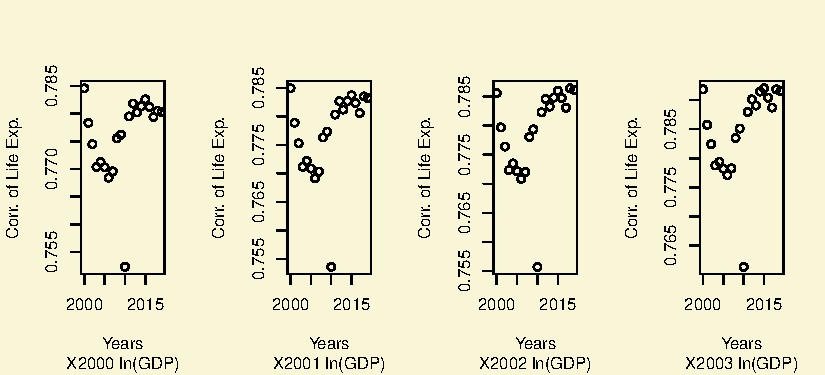
\includegraphics{main_files/figure-pdf/unnamed-chunk-27-1.pdf}

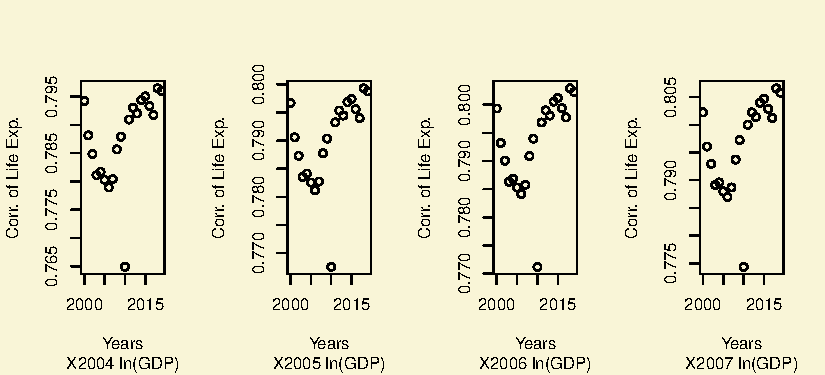
\includegraphics{main_files/figure-pdf/unnamed-chunk-27-2.pdf}

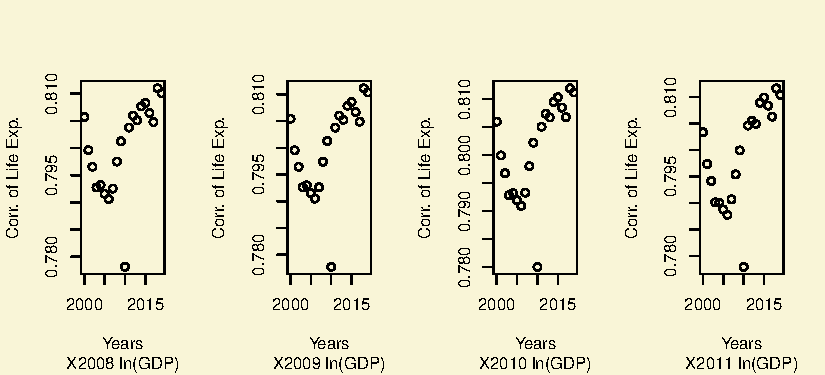
\includegraphics{main_files/figure-pdf/unnamed-chunk-27-3.pdf}

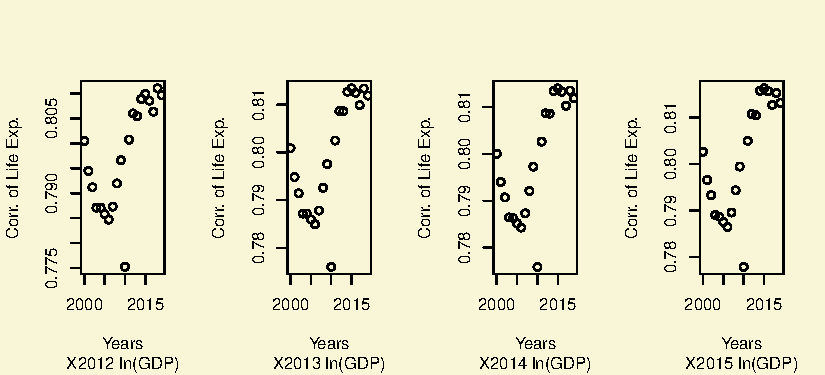
\includegraphics{main_files/figure-pdf/unnamed-chunk-27-4.pdf}

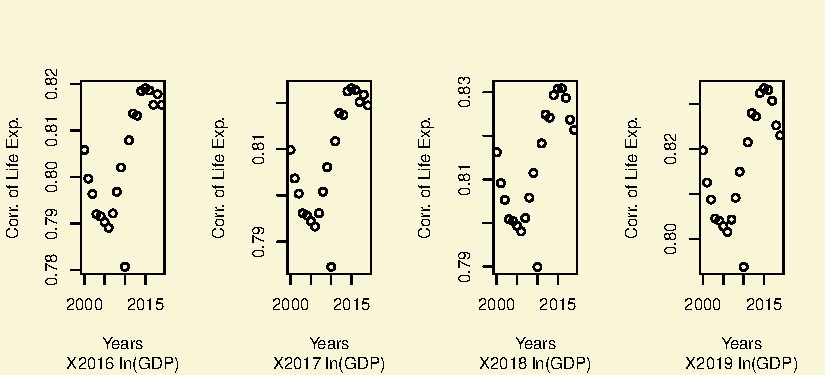
\includegraphics{main_files/figure-pdf/unnamed-chunk-27-5.pdf}

How the years' life expectancies and an year's Sanitation correlate
with.

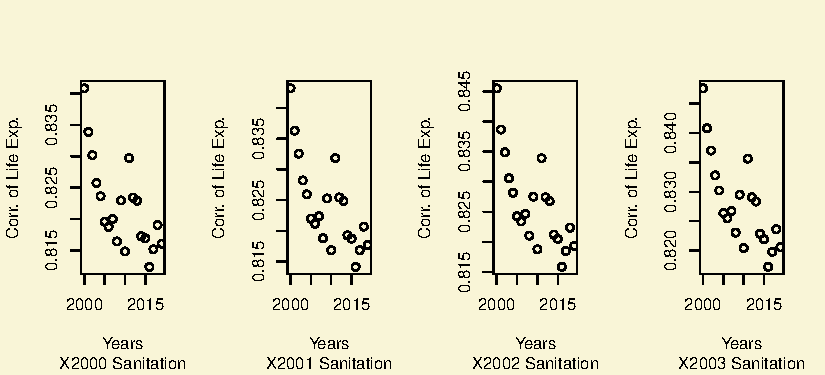
\includegraphics{main_files/figure-pdf/unnamed-chunk-28-1.pdf}

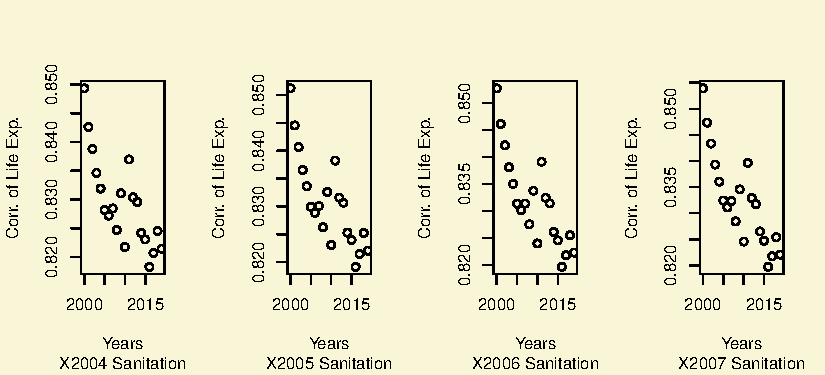
\includegraphics{main_files/figure-pdf/unnamed-chunk-28-2.pdf}

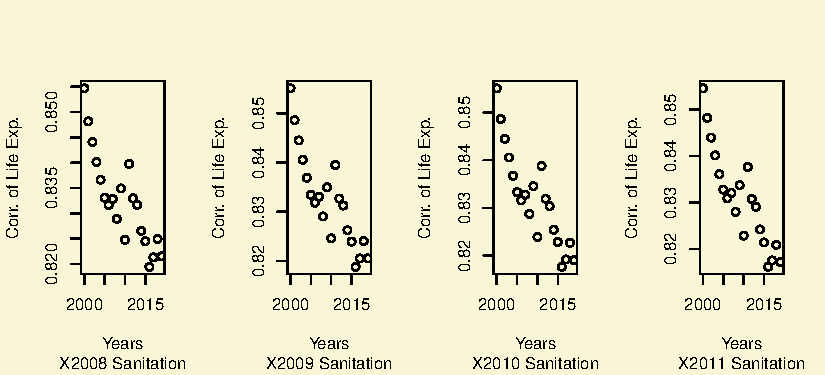
\includegraphics{main_files/figure-pdf/unnamed-chunk-28-3.pdf}

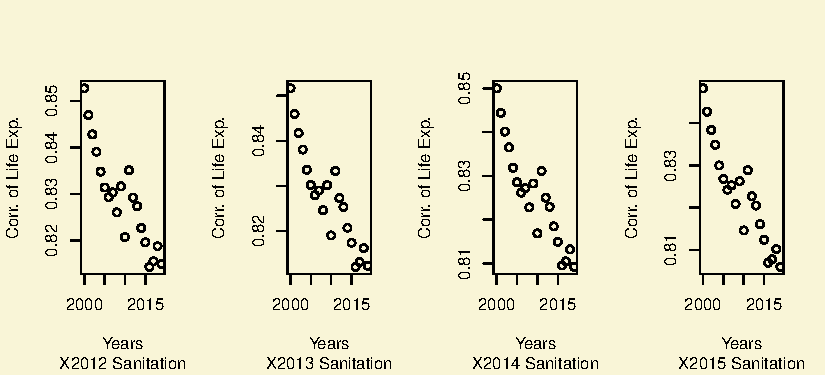
\includegraphics{main_files/figure-pdf/unnamed-chunk-28-4.pdf}

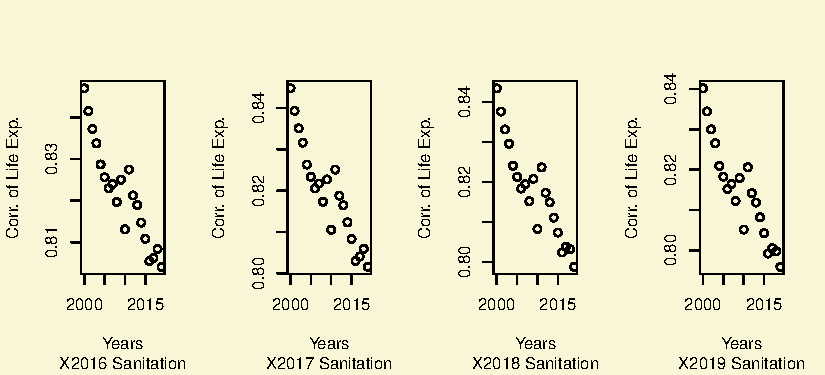
\includegraphics{main_files/figure-pdf/unnamed-chunk-28-5.pdf}

How an year's life expectancies correlate with the years' GDP.

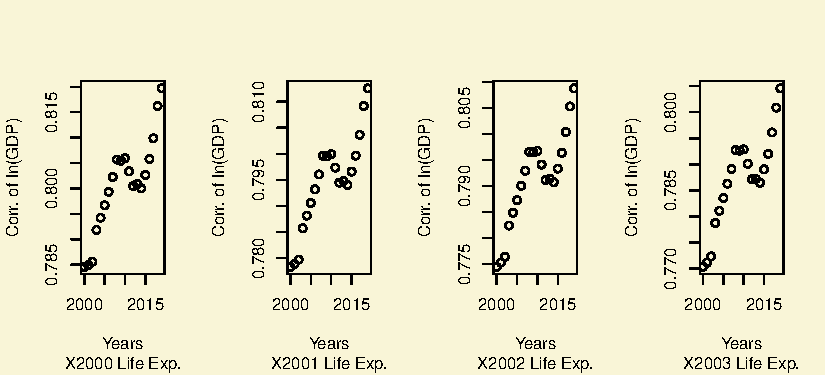
\includegraphics{main_files/figure-pdf/unnamed-chunk-29-1.pdf}

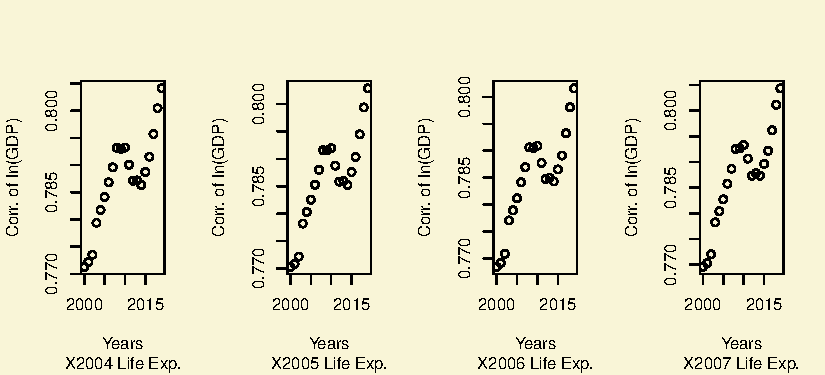
\includegraphics{main_files/figure-pdf/unnamed-chunk-29-2.pdf}

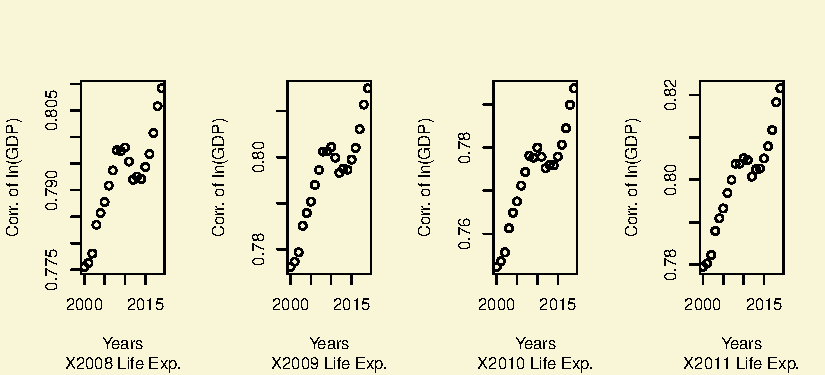
\includegraphics{main_files/figure-pdf/unnamed-chunk-29-3.pdf}

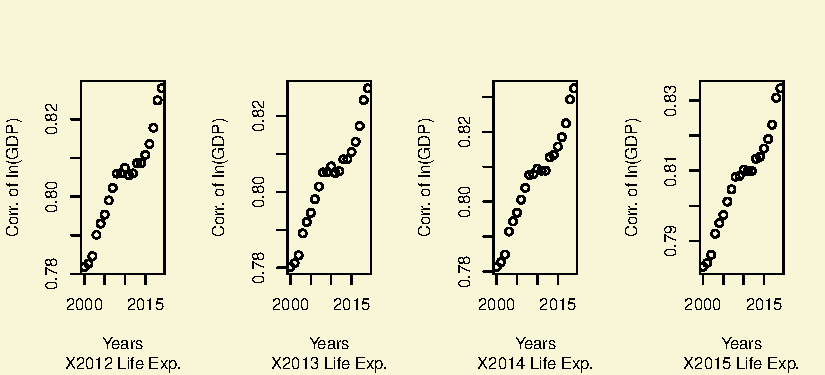
\includegraphics{main_files/figure-pdf/unnamed-chunk-29-4.pdf}

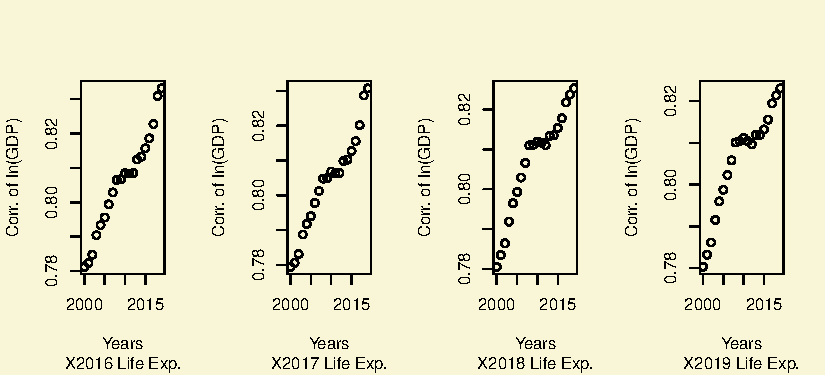
\includegraphics{main_files/figure-pdf/unnamed-chunk-29-5.pdf}

How an year's life expectancies correlate with the years' Sanitation.

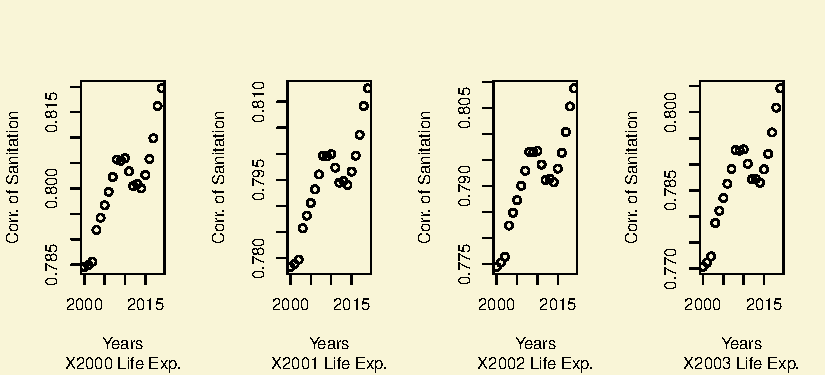
\includegraphics{main_files/figure-pdf/unnamed-chunk-30-1.pdf}

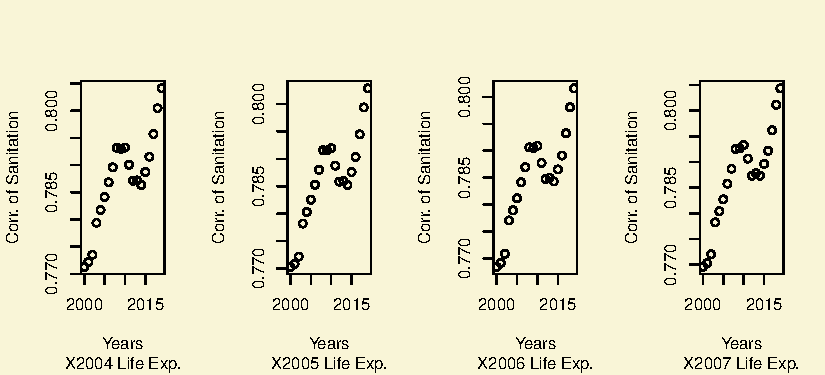
\includegraphics{main_files/figure-pdf/unnamed-chunk-30-2.pdf}

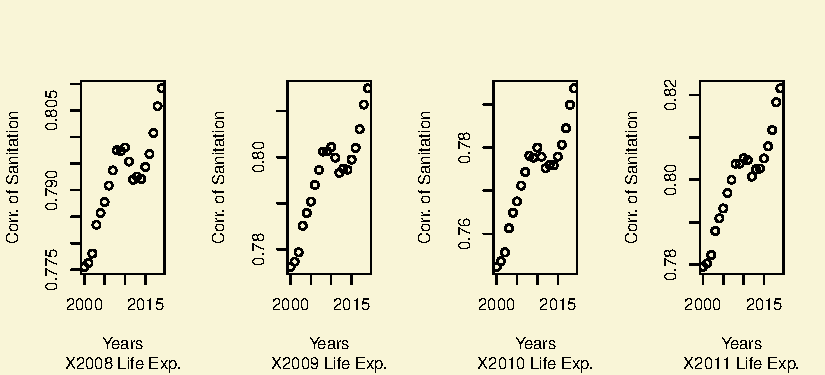
\includegraphics{main_files/figure-pdf/unnamed-chunk-30-3.pdf}

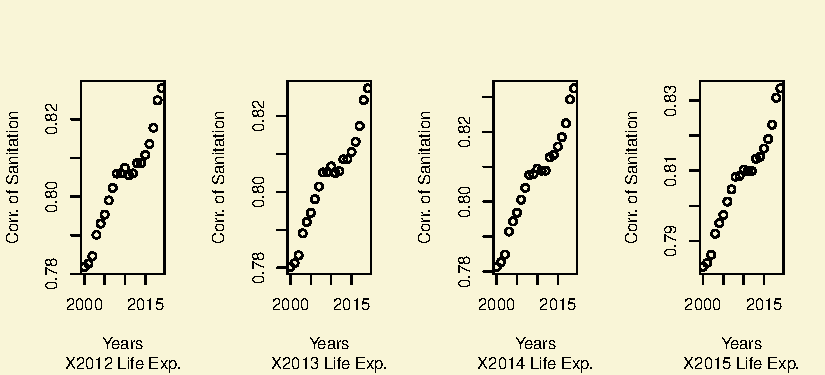
\includegraphics{main_files/figure-pdf/unnamed-chunk-30-4.pdf}

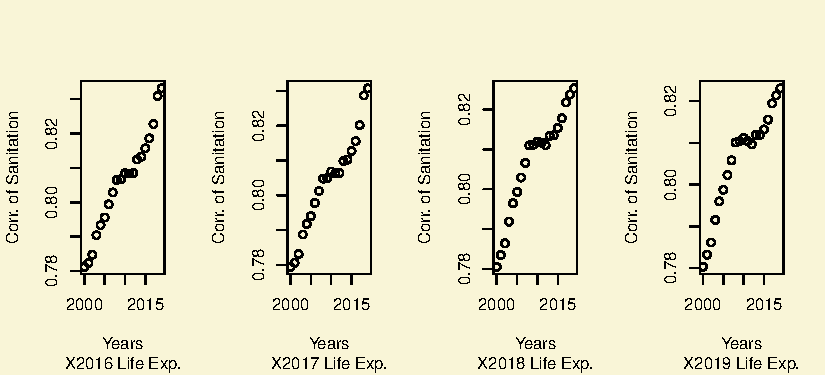
\includegraphics{main_files/figure-pdf/unnamed-chunk-30-5.pdf}

Thus our analysis is fairly robust with respect to variation in Time.
Thus we only perform the analysis on the year 2010.

\hypertarget{raw-gdp-per-capita}{%
\subsection{Raw GDP per capita}\label{raw-gdp-per-capita}}

Sanitation vs GDP per capita

Life Expectancy vs GDP per capita

Scatter Plots of Sanitation or Life Exp. with respect to raw GDP are not
linearly correlated. As this was beyond our scope of knowledge, we
instead considered the log (base \(e\)) of GDP.

Thus in reality, rise in GDP provides diminishing returns in citizen
health the wealthier a country is.

\hypertarget{conclusion}{%
\section{Conclusion}\label{conclusion}}

Thus we have observed that Life expectancy increases with rise in log of
GDP per capita and Sanitation facility access. Life Expectancy is also
more directly affected by increase in basic Sanitation access than with
rise in log of GDP per capita.

\hypertarget{suggestions}{%
\subsection{Suggestions}\label{suggestions}}

Governments should consider that:

\begin{itemize}
\item
  Focusing on better sanitation services leads to visibly better
  lifespan of the citizens.
\item
  Improvements in GDP per capita make practical improvements in
  sanitation and life expectancy only for poorer countries, due
  diminishing returns in the log scale.
\item
  Improvements to life expectancies once made, are fairly stable.
\end{itemize}

\hypertarget{notable-countries}{%
\subsection{Notable Countries}\label{notable-countries}}

Some countries had alarmingly low Life Expectancies:

\begin{itemize}
\item
  The countries like the Central African Republic, Zimbabwe have very
  low life expectancies due to endemic poverty and weak governance,
  contributing to a dire health situation.
\item
  Haiti had a high child mortality rate in 2010 due to natural disasters
  and cholera outbreaks. This caused low Life expectancy for that year.
\end{itemize}

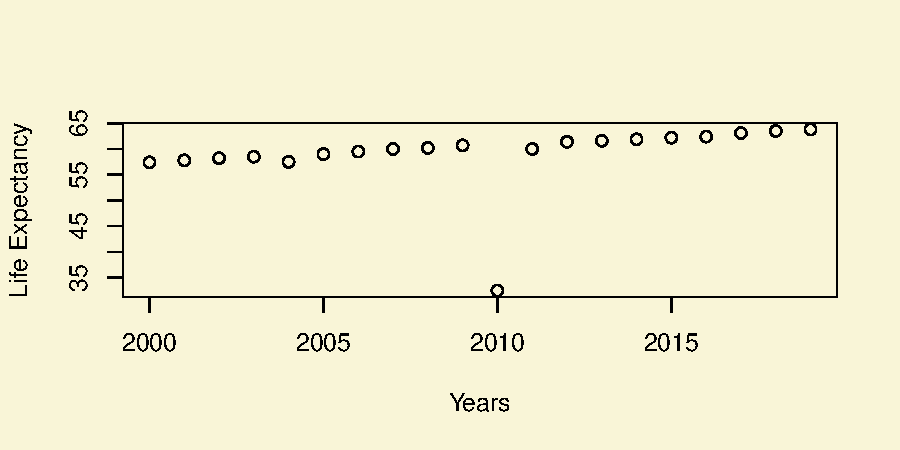
\includegraphics{main_files/figure-pdf/unnamed-chunk-33-1.pdf}

\begin{itemize}
\tightlist
\item
  Countries like Mozambique, Lesotho are experiencing increasing double
  burden of diseases characterized by an increase in the burden of
  non-communicable diseases as well as a high burden of communicable
  diseases.
\item
  Also countries like Eswatini, Zambia also have a low life expectancy
  due to the outbreak of HIV.
\end{itemize}

\hypertarget{credits}{%
\section{Credits}\label{credits}}

\begin{itemize}
\tightlist
\item
  Dr.~Kiranmoy Das
\item
  \href{https://gapminder.org}{Gapminder}
\item
  \href{https://wikipedia.org}{Wikipedia}
\item
  \href{https://statology.org}{Statology}
\item
  \href{https://quarto.org}{Quarto}
\item
  \href{https://posit.co/products/open-source/rstudio/}{RStudio}
\end{itemize}

\hypertarget{thank-you}{%
\section{Thank You}\label{thank-you}}



\end{document}
